\documentclass[12pt]{article}
\usepackage[top=1in, bottom=1in, left=1in, right=1in]{geometry}
\usepackage{setspace}
\usepackage{amsmath}
\usepackage{amssymb}
\usepackage{url}
\usepackage{graphicx}
\usepackage{natbib}
\usepackage[    pdftex,                     hyperfootnotes=true,       colorlinks=true,            citecolor=black,             linkcolor=black,             urlcolor=blue,              breaklinks=true             ]{hyperref}

\parskip=0pt
\parindent=30pt
\begin{document}

\date{\today}
\title{Legal Institutions and Oppressive State Violence or: All the Crimes Committed, Day by Day}
\author{Andreas Beger\thanks{Predictive Heuristics. email: \href{mailto:adbeger@gmail.com}{adbeger@gmail.com}.} \\
Daniel W. Hill, Jr.\thanks{Assistant Professor, Department of International Affairs, University of Georgia. email: \href{mailto:dwhill@uga.edu}{dwhill@uga.edu}.}}

\maketitle 

\begin{abstract}

\end{abstract}

\clearpage
\setcounter{page}{1}

\doublespace

\section*{Introduction}

Modern states are the most powerful organizations that have ever existed. Such organizations can serve the valuable purposes of creating basic social order and facilitating the provision of public goods, among others. But every state also poses a potential threat to those that live in its territorial jurisdiction. Any organization powerful enough to enforce laws and collect taxes also has the ability to use its coercive capacity against the public, and will at least occasionally be tempted to do so. Indeed, the creation of social order and the extraction of wealth (even for public goods provision) are both inherently coercive, and abuses of authority may occur during the course of these activities. The question of how to design a government that wields tremendous coercive power but does not abuse that power is central to contractarian theories of government, which date back at least to Hobbes. 

Much more recently (since the late 1980s), there has emerged a strand of quantitative political science that speaks directly to this question. There is now a large, rich literature that examines government abuses of ``physical integrity,'' which include egregious abuses of power such as arbitrary imprisonment, torture, and extralegal detention and execution. Made possible by the creation of a variety of quantitative indicators of government violence, this body of research has uncovered a number of reliable patterns in the data. As a result, we now know far more about the conditions under which state agents are more or less likely to engage in violent abuses of authority, and whether/how various political and legal institutions can mitigate these abuses. For example, mass political participation, political competition, constraints on executive discretion over policy (including an independent judiciary), constitutional guarantees for certain rights, and the nature of the domestic legal system are all negatively associated with physical integrity abuse \citep[E.g.,][]{PoeTate1994,Davenport1996,Poeetal1999,BdMetal2005,Davenport2007,KeithTatePoe2009,Mitchell2013,HillJones2014}.   

Although progress and accumulation in this literature are apparent, there is still much that we do not know. The vast majority of existing arguments focus squarely on repression \citep{Haschke2011}, defined as state violence that targets organized political opposition or that is meant to raise the cost of organized resistance \citep{Bisselletal1978,Tilly1978, Goldstein1978, StohlLopez1984,Davenport2007AR}. The first wave of the literature was largely decision-theoretic and focused on a political leader's choice to use violence. These accounts treated violence as a policy option that leaders use when the political threat of dissent exceeds the expected cost of violent repression \citep{Davenport1995,Poe2004}. More recent, strategic accounts of state violence also theorize primarily about violence as a tool for minimizing domestic political threats \citep{Pierskalla2010,Ritter2014,RitterConrad2016}. 
It is not surprising that political scientists have paid the most attention to government violence related to political competition, i.e.\ repression. But quelling dissent is only one of several reasons that state agents use violence. This means that explanations for violence that focus exclusively or primarily on repression are missing a large part of the picture. 

One need look no farther than existing data on government violence to appreciate that abuse of personal integrity is a broad category that includes more than the repression of dissent. The most commonly used indicators of violence are based on content analyses of human rights reports issued annually by the US State Department and Amnesty International \citep{CIRI2014, PTS2015}. Perusing these reports, it is not difficult to find statements such as this, from Amnesty's 1985 report on Brazil:
\begin{quote} 
Throughout 1985 the Brazilian press carried allegations of torture and ill-treatment of criminal suspects and prisoners, many of whom were minors.
\end{quote} 
Or this, from the 1995 report on Greece:
\begin{quote}
\ldots prisoners in Greek police stations suffered ``severe ill-treatment'' by officers using hand-held electric shock devices, according to a November 1994 report of the Council of Europe's European Committee for the Prevention of Torture and Inhuman or Degrading Treatment or Punishment.
\end{quote} 
Or this, from the 2005 report on Albania: 
\begin{quote}
Police officers or prison guards allegedly beat detainees during arrest or subsequently in detention. At least six such complaints, three of them made by taxi-drivers, related to police officers attached to Korpe police station.
\end{quote}
In each of these cases the victims are not apparently involved in any explicitly political activity that threatens the state's authority. From the standpoint of most explanations of physical integrity abuse, then, the motive for abuse in each case is unclear. A more systematic examination of the data, presented below, suggests that the kinds of incidents recounted above are at least as common as incidents where people are targeted by state agents for their (perceived) political activities or affiliations. One of our purposes is to call attention to the diversity of abuses included in the category ``physical integrity violation.'' We refer to state violence used to suppress or prevent political opposition as ``repressive'' violence, and state violence unrelated to political challenges as ``oppressive'' violence \citep{Bisselletal1978}. We believe that drawing a distinction between politically motivated abuse and abuse without clear political motivations will be useful conceptually and empirically. Conceptually, distinguishing between the repression of dissent and the kind of violence described in the three examples above is necessary to develop more complete explanations of personal integrity abuse. Arguments that assume violence is intended to diminish domestic political threats do not apply as clearly to oppressive violence, as the victims pose no threat to the government's tenure. Empirically, expanding our explanations to consider violence beyond repression will allow us to more accurately model and predict patterns of government violence. Our theories are intended to explain only part of what we are able observe, but are applied to all of what we are able to observe. Thus, it seems likely that these theories, and the empirical models they motivate, do not describe or capture the world as accurately as they could.   

Since repressive and oppressive violence have different underlying motives, they are likely to require different solutions. Domestic political and legal institutions, primarily those related to democracy and institutional constraints on executives, have received much attention in the literature. We argue that the mechanisms by which these institutions are thought to constrain state agents are more likely to operate for repressive violence than for oppressive violence. Domestic institutions are thought to limit abuse because they make political leaders accountable to the public and make it easier for the public to coordinate opposition to abuse, broadly defined. However, public backlash and coordination is much less likely in response to cases of oppressive violence. For this category of violence, domestic institutions can limit abuse not because they create opportunities for broad political action but rather because they create explicit, actionable rights for individuals that can be enforced by courts. Explicit rules that protect potential victims, and legal systems that are conducive to their enforcement, can reduce the risk to individuals of being detained by the state in the first place, and also make it more likely that agents responsible for violent abuse are caught and punished.    

Our paper proceeds as follows. In the next section, we discuss further the distinction between repressive and oppressive physical integrity violations, and discuss some basic descriptive statistics that speak to their prevalence. We next develop an argument about the effectiveness of political and legal institutions at reducing their occurrence, drawing on existing theories of domestic institutions and government violence. We then conduct an analysis that distinguishes between repressive and oppressive violence and allows us to determine whether institutions known to mitigate repressive violence have similar effects on oppressive violence. In our analysis we also examine the in- and out-of-sample accuracy of statistical models that use legal and political institutions to predict violence.    

\section*{Repressive and Oppressive Violence} 

Responding to (or preempting) dissent is one reason that governments use violence against the public. But not all state violence targets people who the government perceives as threatening to its authority. In many cases the victims are criminal suspects or convicted criminals who are abused by the police under the guise of ``social order.''  For example, in his book on torture in democracies \citep{Rejali2007} discusses the prevalence of police torture in the Japanese criminal justice system. Here the victims are criminal suspects. Police have wide discretion over where and how long they detain suspects, and tend to rely heavily on confessions as a form of evidence. Consequently, torture during pre-arrest detention is relatively common. \citep{Rejali2007} discusses an additional kind of torture that is unrelated to political threats. His ``civic discipline model'' describes a situation in which and informal agreement exists between citizens and the police (or private security firms). Police provide ``law and order'' by using violence to demarcate social-geographic boundaries, i.e. to keep ``undesirables'' out of certain areas, and the public ignores police violence as long as it achieves this goal. 
%He argues that its high frequency is the result of an excessive reliance on confessions rather than physical evidence in criminal trials, and legal rules that allow police to easily prolong pre-arrest detention periods. A combination of wide discretion about detainee treatment and professional incentives to produce evidence results in routinized torture. 
%His ``juridical model'' also seems to apply well to cases like Jon Burge's use of torture over two decades in Chicago. Burge and others, convinced of suspects' guilt and eager to produce evidence, used torture to extract confessions that, in many cases, led to convictions in court. Some of these convictions were overturned (years later) after investigation revealed the role of torture in the confessions. In Chicago police designed an extralegal system to circumvent rules prohibiting prolonged detention. 

In one sense, government violence that targets non-dissidents has been largely ignored in the quantitative, cross-national literature on state violence. The {\em arguments} in this literature speak mostly to violence used to suppress dissent. But the data analyzed in most of these studies includes much violence that is more oppressive in nature, which is readily apparent from reading the human rights reports from which these data are coded. In order to separate out these distinct kinds of government violence, we take advantage of a relatively new data collection effort: the Ill-Treatment and Torture Data Collection Project \citep{ConradHaglundMoore2014}. 

The ITT data catalogues allegations of torture by Amnesty International from 1995-2005 (inclusive). These allegations come from AI's annual reports, action reports, and press releases. This study relies on ITT's Specific Allegations data, which contains information about 16,431 individual allegations of state torture. In each event there is a victim who is in the custody of a state agent (the perpetrator), and an act of violence that meets the international legal definition of torture.\footnote{The definition comes from The United Nations' Convention Against Torture and Other Cruel, Inhuman or Degrading Treatment or Punishment (CAT).} Whereas previous data on government violence did not distinguish between repressive and oppressive violence, the ITT data include information on the identity type of the victim, which allows us to examine the abuse of dissidents separately from other types of victims. 

Descriptive statistics from the ITT specific allegations data suggest that oppressive violence is at least as common as, or perhaps more common than, repressive violence. The ITT uses a typology of victims based on the information contained in AI's reports. Though Amnesty International began with the goal of calling attention to political prisoners, it has been conducting a ``Campaign Against Torture'' since 1972. The organization's broad goal is to publicize abuse where it finds credible evidence of abuse having occurred. As such, AI's reports are not limited to politically motivated violence, but contain allegations of abuse that targets a diverse range of people. Dissident is one of the victim types used in the ITT data, but there are several others, including criminal, member of a marginalized social group, state agent, prisoner of war, and unstated, meaning the allegation does not identify a victim type. Figure \ref{victims} shows the frequency of each victim type in the data. 

In 4,211 of 16,431 allegations in ITT (or about 26\%), the victim's identity type is not mentioned, making ``unstated'' the most common category of victim. For allegations that list a victim identity, the identity may correspond to more than one category, which is the case in 2,704 allegations (16.5\%). Among allegations with a unique, identified victim type, dissidents account for 31\% of allegations, and are the second most common victim type after members of marginalized groups (38.8\%).\footnote{The ITT defines a member of a marginalized social as someone who ``is tortured by the state for the purpose of social control (i.e., humiliation or other punishment to establish that [1] her/his behavior was inappropriate and [2] that the state can abuse her/him with impunity), rather than for the collection of information.'' It lists as candidates immigrants, asylum seekers, the homeless, geeks, punks, skinheads, as well as minorities, e.g.\ sexual and national (ITT Codebook, p.\ 25--26).} Criminals account for 27.7\% of these allegations, while POWs and state agents combined account for less than 3\%. If we add to our count of dissident allegations cases where the victim falls into the dissident category and at least one other category, then allegations involving the torture of dissidents make up about 38\% of all of the events in ITT with an identified victim type. Of all of the instances of torture publicized by AI between 1995-2005 where the identify of the victim was mentioned, the victim was not a dissident about 62\% of the time. 

The ITT data do not constitute a census of cases of torture. Its creators encourage users to treat the data as what they are, {\em allegations} of torture, rather than a count of cases of torture.\footnote{See \citet{HillMooreMukherjee2013} for an analysis of the CIRI torture scale that accounts for the process by which AI produces information about torture. See also \citet{ConradHillMoore} who analyze the ITT data using a model that accounts for this process. It should be noted that the validity of the ITT data as a measure of actual torture is at least as strong as existing torture scales, which are created from a very similar (or the same) set of documents, but contain less information about the abuse described in those documents.} Nevertheless, an examination of the allegations themselves can be instructive for our immediate purpose, which is simply to show that state violence extends well beyond the abuse of dissidents. Taking ITT as an indication, it is plausible that oppressive violence constitutes a non-trivial portion of all personal integrity abuse. This means that explanations for state violence that focus on the repression of dissent leave many cases of violence unexplained. 

Though the explanations in the literature are tailored mainly to repression, most cross-national analyses use data coded from sources that include accounts of oppressive violence.\footnote{The two most commonly used indicators are the Political Terror Scale and the Cingranelli-Richards physical integrity scale. Both are created from content analyses of human rights reports from AI and USSD. PTS also includes HRW.} As mentioned above, these studies have uncovered some reliable patterns in the data. Economic development, for example, is negatively correlated with violations of personal integrity in nearly every study. Perhaps this suggests that the distinct types of violence we discuss here have similar determinants. If this were the case, it would be fair to ask what we gain by considering them separately. We believe such an analysis is warranted for several reasons. First, the distinct types of state violence we discuss have different underlying motives. There is good reason to believe that they do not have the same preconditions, and that particular political and legal institutions do not constrain their use to the same extent, a point we elaborate in the next section. Second, if our argument is correct, then we can more accurately explain and predict different types of state violence if we analyze and model them separately. Finally, we cannot know whether this is the case unless we disaggregate them and consider them separately. It will be useful to know whether explanations for repression apply reasonably well to non-politically motivated state violence. If they do, then we can usefully analyze them together and perhaps develop more general explanations for state violence. If they do not, then more data collection efforts that distinguish between different kinds of violence will be necessary. Such efforts will allow us to develop and test more specific explanations for different kinds of violence, and learn which institutions are effective at preventing each.     

\section*{Domestic Institutions and State Violence}

\subsection*{The Limits of Domestic Institutions}
One of the strongest findings in the literature is that democratic political institutions are negatively associated with violations of physical integrity, with the caveat that democracy has a smaller constraining effect in the presence of violent dissent \citep{Davenport2007AR,Davenport2007}. Here democracy most often refers to high levels of participation and inter-group competition (Dahl). The most straightforward argument for why democracy would reduce abuse is that elected officials in democracies are agents of the public who can be removed for bad policy outcomes. Competitive elections provide a low-cost way for the public to get rid of leaders who instigate or allow widespread abuse.\footnote{This is finding is partly due to the fact that violence against political opposition groups constitutes a violation of democratic principles as well as personal integrity, so that the definitions overlap to some extent \citep{HillJones2014,Hill2016}.}  

However, there are reasons to doubt that the public will respond this way to physical integrity abuse. Building on Walzer's (1973) \nocite{Walzer1973} argument about ``dirty hands,'' \citet{Moore2010} argues that participation/competition is a relatively weak constraint on violence that targets minority groups. In democracies, the public expects political leaders to by hypocrites. They hold the government  accountable for providing public security, and expect them to commit human rights abuses in the name of security, but also to publicly deny that any abuse has occurred. Moore argues that leaders may even be able to publicly acknowledge using torture and avoid electoral punishment. Since torture typically targets small, marginalized groups who the general public perceives as threatening \citep{Rejali2007}, elected leaders pay no political cost if its use becomes known to the public \citep{ConradHillMoore}. 

Apart from accountability to the public, another reason political competition may reduce violence is that regular leadership turnover reduces elites' incentive to seize or maintain power through violence. This is because regular turnover lowers the costs of losing office; today's losers may be tomorrow's winners. The outcome of a violent political contest, on the other hand, is often highly uncertain. When it is sufficiently uncertain, the expected cost of using violence to retain power exceeds the cost of peacefully conceding \citep{Przeworski1991}. 

Another line of argument calls attention to the ability of certain political institutions to aid the public in coordinating a response to government abuse. Here government abuse is broadly defined to include actions such as arbitrary arrest or confiscation of property, torture, violations of constitutional law, and violations of existing rules about political succession. This strand of the literature also views elections as useful for this purpose \citep[E.g.,][]{Fearon2011}, but focuses primarily on formal protection for individual rights and strong/independent courts of law \citep{NorthWeingast1989,Weingast1997,Vanberg2005,ElkinsGinsburgMelton2009,PowellStaton2009,Melton2013}. Citizens who wish to oppose abuse face a coordination problem. Opposition must be widespread to be effective, but due to uncertainty about how others will respond and the potentially high cost of participating in political action, generating widespread opposition is difficult. Formal rules (e.g., constitutions) aid coordination by providing a common definition of ``abuse,'' which can reduce uncertainty about how others will respond to particular government actions. Courts of law make coordination less difficult still, because they provide information about abuse to the public. High courts in particular provide a prominent, visible signal that abuse has/has not occurred. All of this suggests that formal protections for individual rights, and strong courts of law, should be associated with less frequent government abuse, included abuse of physical integrity. 

One of our theoretical claims is that these arguments apply more readily to politically motivated violence than they do to oppressive violence. Przeworski's (1991) argument quite clearly applies only to violence that is used to claim or maintain political power. Settling political contests with violence is risky, but there is nothing in this account that suggests that competition creates incentives for political leaders to refrain from abusing groups beyond political opponents.  

Arguments about electoral accountability and institutions as focal points for coordination also apply more readily to repressive violence. These arguments are closely connected; in both cases, the mechanism that curbs physical integrity violations is the anticipation of public backlash in response to abuse. Elections, constitutions, and courts of law provide information that allows the public to determine whether abuse has occurred, which creates an opportunity for mass action to remove abusive governments. In this framework, the public has a interest in removing leaders who violate the social pact because abuses of authority are detrimental to their welfare. Recall Moore's (2010) point that the general public does not particularly care about the welfare of the groups most likely to be victims of torture. This dovetails with one of the insights from \citet{Weingast1997}. The public is not an undifferentiated mass, but consists of multiple groups with different interests, some of whom may not be affected by the abuse of others or may actually benefit from it. If abuse is targeted rather than indiscriminate, then for an individual member of the public to respond it must be the case that they anticipate being the victim of abuse at some point in the future. When this is the case, and members of the public use punishment strategies to sanction individuals who do not oppose abuse, mass coordination in response to abuse is a stable outcome. The basic idea is that the group that escapes abuse today may become victims in the future, in which case they will require the help of today's victims, which gives them incentive to oppose the abuse of others. 

This reasoning suggests that these institutions are of limited usefulness for preventing oppressive violence. Consider first the case of repressive violence, which in many cases targets people for exercising basic political rights, i.e.\ openly supporting political opposition groups. It seems plausible that the mechanism described above can effectively prevent this kind of abuse. This is for the simple reason that ``supporter of an organized political group'' is a category to which many members of the public belong, if ``support'' includes merely openly sharing the policy preferences of a particular group. As a consequence, it is easy for an individual to imagine that violence against supporters of political groups may affect them. Many people can imagine themselves being in the political minority, voting for a losing candidate, etc. After all, even for supporters of the current government, given regular turnover in leadership there is some chance that they will be in the ``opposition'' in the future. This is precisely the point Przeworski makes, applied to the public rather than political elites. These arguments are partly about the maintenance of democracy itself; all of these institutions reduce a government's incentive to forego peaceful competition and forcibly subdue their political opponents.  

On the other hand, these institutions only go so far towards reducing abuse that targets groups who members of the public do not readily identify with. Oppressive violence targets victims for reasons other than their political preferences, and victims of such violence typically belong to groups that are, by definition, a minority of the population: criminal suspects, immigrants, members of ethnic minorities, etc. Institutions that provide a low cost mechanism for opposing abuse will not matter when the public has no incentive to respond to abuse. And, since the average member of the public is more likely to identify as supporter of a political group than they are as, e.g.\, an immigrant, violence that targets the latter group is less likely to trigger a response from the average member of the public. Knowing this, political leaders will not be especially concerned about backlash in the wake of abuse that targets these groups. Consider the recent spate of extralegal executions in the Philippines. Since coming to power in the Summer of 2016, President Rodrigo Duterte has implemented anti-drug policies that have resulted in thousands of illegal killings by the national police.\footnote{\url{https://www.hrw.org/news/2017/09/07/philippine-president-rodrigo-dutertes-war-drugs}} In fact, Duterte {\em campaigned} on his hard-line stance against drug users and sellers, and had developed a reputation for being ``tough on crime'' during his years as Mayor of Davao City. Though the killing of a high school student last summer caused some public backlash against these policies, the policies are still in place, and Duterte enjoys high public approval ratings according to the latest polls. 
%In his study of torture in democracies, \citet{Rejali2007} discusses police torture in the criminal justice system, arguing that it results from reliance on confessions rather than physical evidence in criminal trials, and legal rules that allow police to prolong pre-arrest detention. He also discusses violence that targets people who are not necessarily suspected of any criminal violation, but have transgressed customs concerning social hierarchies based on class, ethnicity, or some other social distinction. \citet{Rejali2007} refers to this as violence in pursuit of ``civic discipline.'' In the same vein as \citet{Walzer1973}, he describes an informal social arrangement between citizens and state agents where citizens demand ``social order'' and turn a blind eye to torture if they believe it accomplishes that goal.  

The discussion above suggests that certain political institutions will be more effective at curbing repressive violence than oppressive violence. To reiterate, this is because the mechanism linking these institutions to reductions in violence depends on the willingness of members of the public to take action against abuse that does not directly affect them. This is much more likely to be the case when victims of abuse belong to a social category with which a large swath of the public identifies. In turn, this is more likely when violence is repressive rather than oppressive.    

\subsection*{A More Optimistic Section}

Despite the limitations discussed above, we believe there are institutional safeguards that can mitigate oppressive violence. In fact, some of the institutions discussed above may be good for this purpose, but not for the reasons typically offered. That is, where oppressive violence is concerned, institutions matter, but not because they facilitate mass political action in response to abuse. Our argument is similar to that of \citet{ConradMoore2010}, who take a slightly different theoretical approach than that outlined in the previous section. Rather than imagining a leader who has to decide whether to abuse rights to achieve some goal, \citet{ConradMoore2010} imagine a leader who takes active measures to prevent abuse, or does not. They start from the premise that state agents will torture at least occasionally if they are not monitored and punished for doing so, and present an argument about how institutions affect a political leader's incentives to stop/prevent torture from occurring. They argue that democratic institutions matter not because public punishes leaders when torture occurs, but because democracy allows citizens to successfully pressure governments to create monitoring/oversight bodies that make torture less likely to occur in the first place. Our argument adopts their focus on the motives of state agents who engage in torture and the political leaders who try to encourage/discourage torture. Institutions can mitigate abuse because they create fewer opportunities and incentives for state agents to use torture, and increase the likelihood that those responsible for abuse are punished. Like Conrad and Moore, we start from the premise that individuals in the custody of the state are at automatically at risk for abuse.\footnote{Here ``custody'' means a state agent has limited an individual's liberty/freedom of movement for some period of time. A person in prison is therefore in the custody of the state, as is someone who has been told to sit on the sidewalk until further instructed.} State agents have various motives for abusing detainees, including interrogation, punishment/social control, and extortion. We do not expect institutions to trigger public outcries on behalf of abused detainees. Instead, we draw attention to legal institutions that help keep individuals out of custody for extended periods of time, and reduce incentives for agents to engage in abuse, either by creating oversight and punishment or by reducing the benefit of using torture on detainees. 

There are several existing studies that examine the relationship between legal institutions and personal integrity abuse, including torture \citep{Davenport1996,Cross1999,Keith2002PRQ,Keith2002,KeithTatePoe2009,PowellStaton2009,RiosStaton2012,ConradRitter2013,Mitchell2013,Conrad2014,HillJones2014,RitterConrad2016}. These studies examine the relationship between state violence and judicial independence/effectiveness, constitutional provisions for individual rights, and legal system type. Our contribution is to develop an argument about, and examine, a broader set of legal rules that we think will be relevant for oppressive violence. We also consider oppressive and repressive violence separately, for the reasons discussed above, in order to examine the differential effects of these legal institutions on repressive and oppressive violence. Our argument is that legal institutions can limit oppressive violence because they 1) minimize opportunities for abuse by limiting the amount of time people spend in state-imposed detention, 2) create conditions conducive to monitoring the state agents most likely to engage in torture, 3) create justiciable rights that entail tangible penalties for individuals who commit abuse, and 4) reduce the incentive for police to use torture in the course of a criminal investigation. 

% work in cites of stuff on judicial independence, and constitutions. Keith, Powell/Staton, Keith/Tate/Poe, Davenport, Cross, Hill/Jones

Taking measures to prevent the state from detaining individuals for long periods of time should curb abuse. This is simply because there will be fewer opportunities for agents to engage in abuse. Many legal rules related to due process are designed to have this effect. Laws that prevent police from holding suspects in custody without a criminal charge, laws that allow for the possibility of pre-trial release, the right to a writ of {\em habeas corpus}, and and laws granting defendants the right to a fast trial create legal obstacles to lengthy detention. Due process rules related to arrest and trial procedure will also help reduce abuse. Here we have in mind laws that prevent police from making arbitrary arrests, as well as laws related to ``fair'' trial procedures. These would include general provisions for fair trials, the right to counsel, the presumption of innocence, and the right of defendants to examine witnesses who testify against them. The nature of the legal system may also be relevant. Legal scholars draw a distinction between adversarial and inquisitorial trial systems. In adversarial systems the court/judge takes no part in the criminal investigation, and instead serves as an impartial party to facilitate the presentation/examination of evidence by the prosecution and defense. In inquisitorial systems the judge does take part in the criminal investigation and may, for example, initiate the examination or presentation of evidence, including interviewing/questioning witnesses. 

Another way that institutions can discourage torture is by creating concrete penalties for those who engage in abuse. We argue that courts of law matter for this reason. Theories of coordination in response to government abuse seem to be concerned primarily with high courts that have the authority to make decisions about whether constitutional rules have been violated by government actors. Our concern, which is more general, is with the ability of courts of law to successfully prosecute/punish state agents responsible for abuse. Like previous studies, we argue that judicial independence/effectiveness can help reduce violations of personal integrity. This is both because independent/powerful courts will be more willing to prosecute state agents and, just as importantly, because strong courts create expectation that victims may actually seek redress \citep{PowellStaton2009}. 

In addition to effective courts of law, we expect that laws explicitly prohibiting torture and related form of abuse will reduce the occurrence of violations. Of course, because formal rules exist does not mean they are followed or enforced. But formal rules create at least the possibility of punishment, and may heighten the expectation of legal punishment. Formal rules also give victims legal grounds to seek redress. Relevant rules here include explicit prohibitions on torture, cruel punishment, and corporal punishment, rules stating there can be no punishment without law, and laws granting victims the right to seek redress in the event that their rights are violated. Additionally, we examine legal provisions that require prisons to keep registries which, where implemented, should make it more difficult for abuse to go undetected. 

Finally, we examine legal rules that reduce the benefit of torturing detainees to state agents. Extracting (false) confessions from criminal suspects is often a motive in police torture. As such, we expect that formal rules declaring coerced confessions to be inadmissible in criminal trials will decrease the police's incentive to use torture in the course of a criminal investigation. 

\section*{Analysis}

The ITT data cover the years 1995 to 2005, 11 years in total. Our data consist of country-years for independent states during that period, following the Gleditsch and Ward list \citep{gleditsch:ward:1999}. This makes for a total of around 1,600 observations. In the raw allegation data, a single allegation may specify any number of six different victim types. We split such multi-victim allegations into seperate allegations for each victim type before counting allegations by country-year-victim type. Figure \ref{fig:victim-types} shows the resulting sum total of allegations for each of the six original victim types. As discussed above, there are few allegations of torture of POWs and state agents, so we leave these out. Some of the descriptive plots will retain the "Unknown" victim type allegations, but since we have no expectations regarding how to apportion these, we will also drop this category for the formal modeling further below. Otherwise, the plot shows that allegations of torture of marginalized and criminal victims are at least as common as allegations of torture of dissidents. 

\begin{figure}
\begin{center}
\caption{}
\label{fig:victim-types}
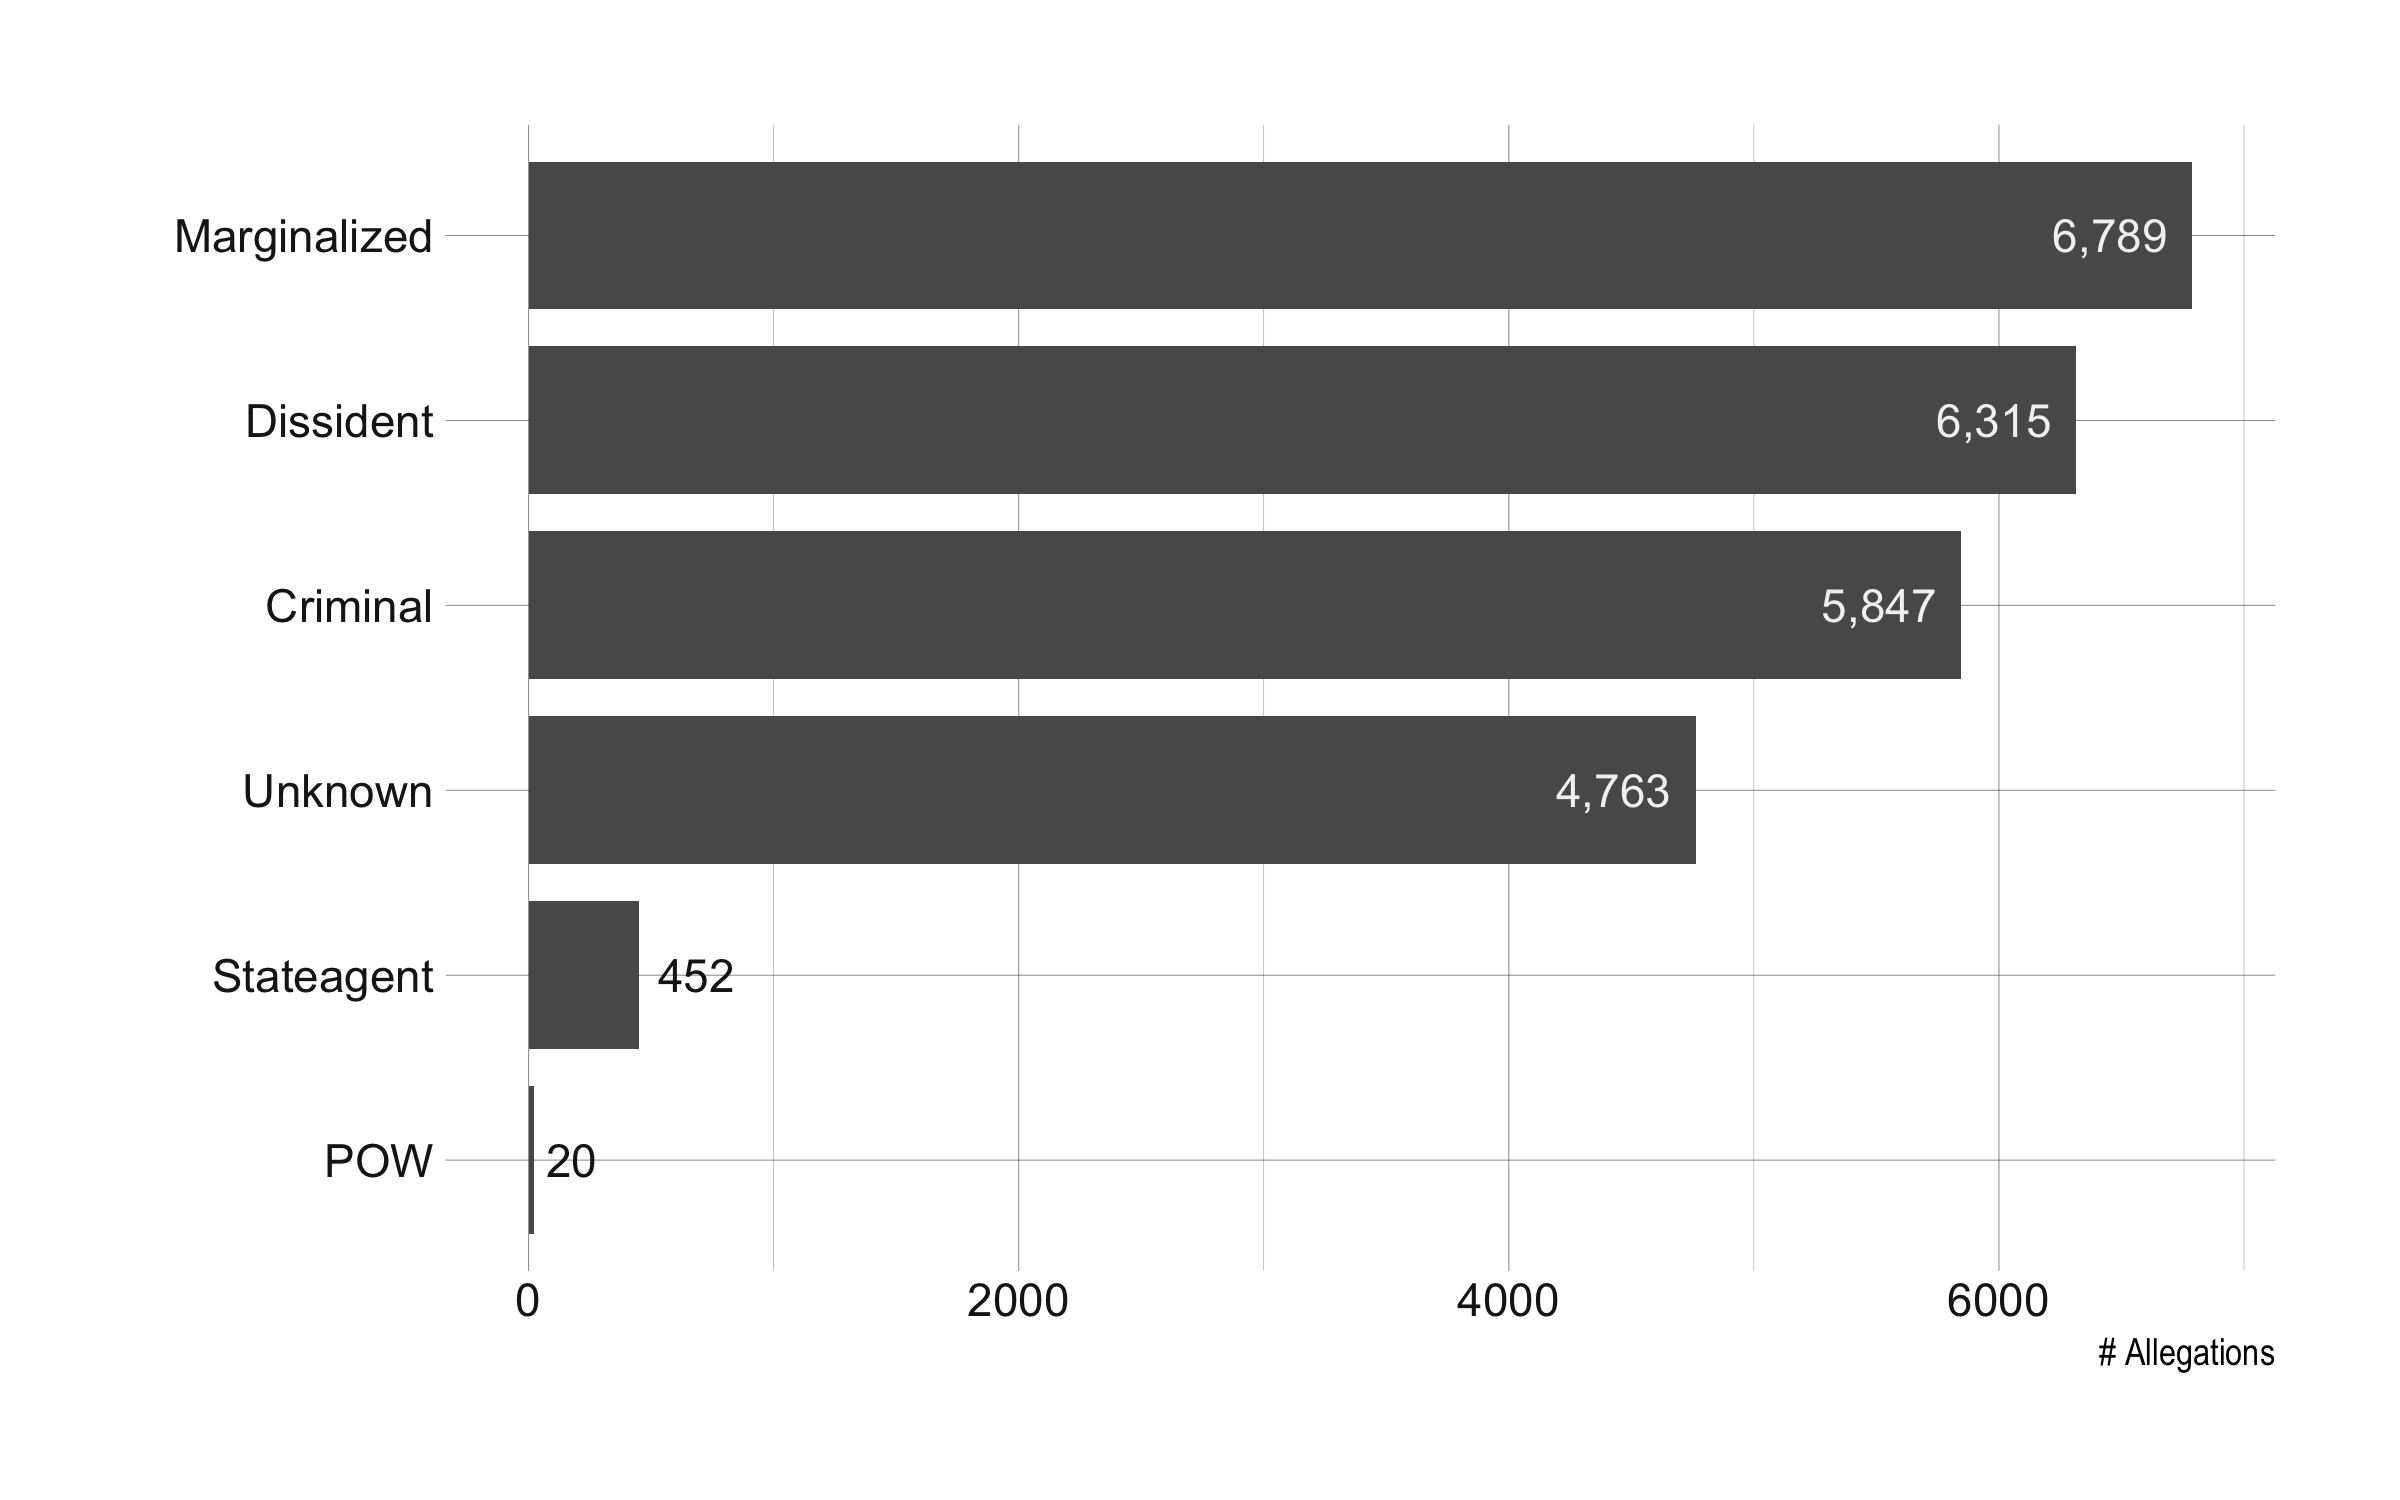
\includegraphics[width=.5\textwidth]{../output/allegations-by-victim.png}
\end{center}
\end{figure}

Figure \ref{fig:selected-series} plots allegation counts for several representative countries. These include Turkey, China, and the US, which have the highest allegation counts overall and the highest counts of allegations of torture of marginalized groups, dissidents, and criminals, respectively. Most countries have few allegations leveled against them at any given time, and in the larger data many country-year-victim type combinations have no allegations at all. Balanced against this are outlying cases like the US and China, with consistently high levels of allegations. Both Turkey and the US have notably more allegations in the 1990's. In the case of Turkey this may correspond to fighting with Kurdish separatists. In any case, there is variation over time that will be hard to explain with relatively constant institutional characteristics. Overall a little bit less than half of the variation in allegation counts is over time, rather than between countries or between victim types. 

\begin{figure}
\begin{center}
\caption{}
\label{fig:selected-series}
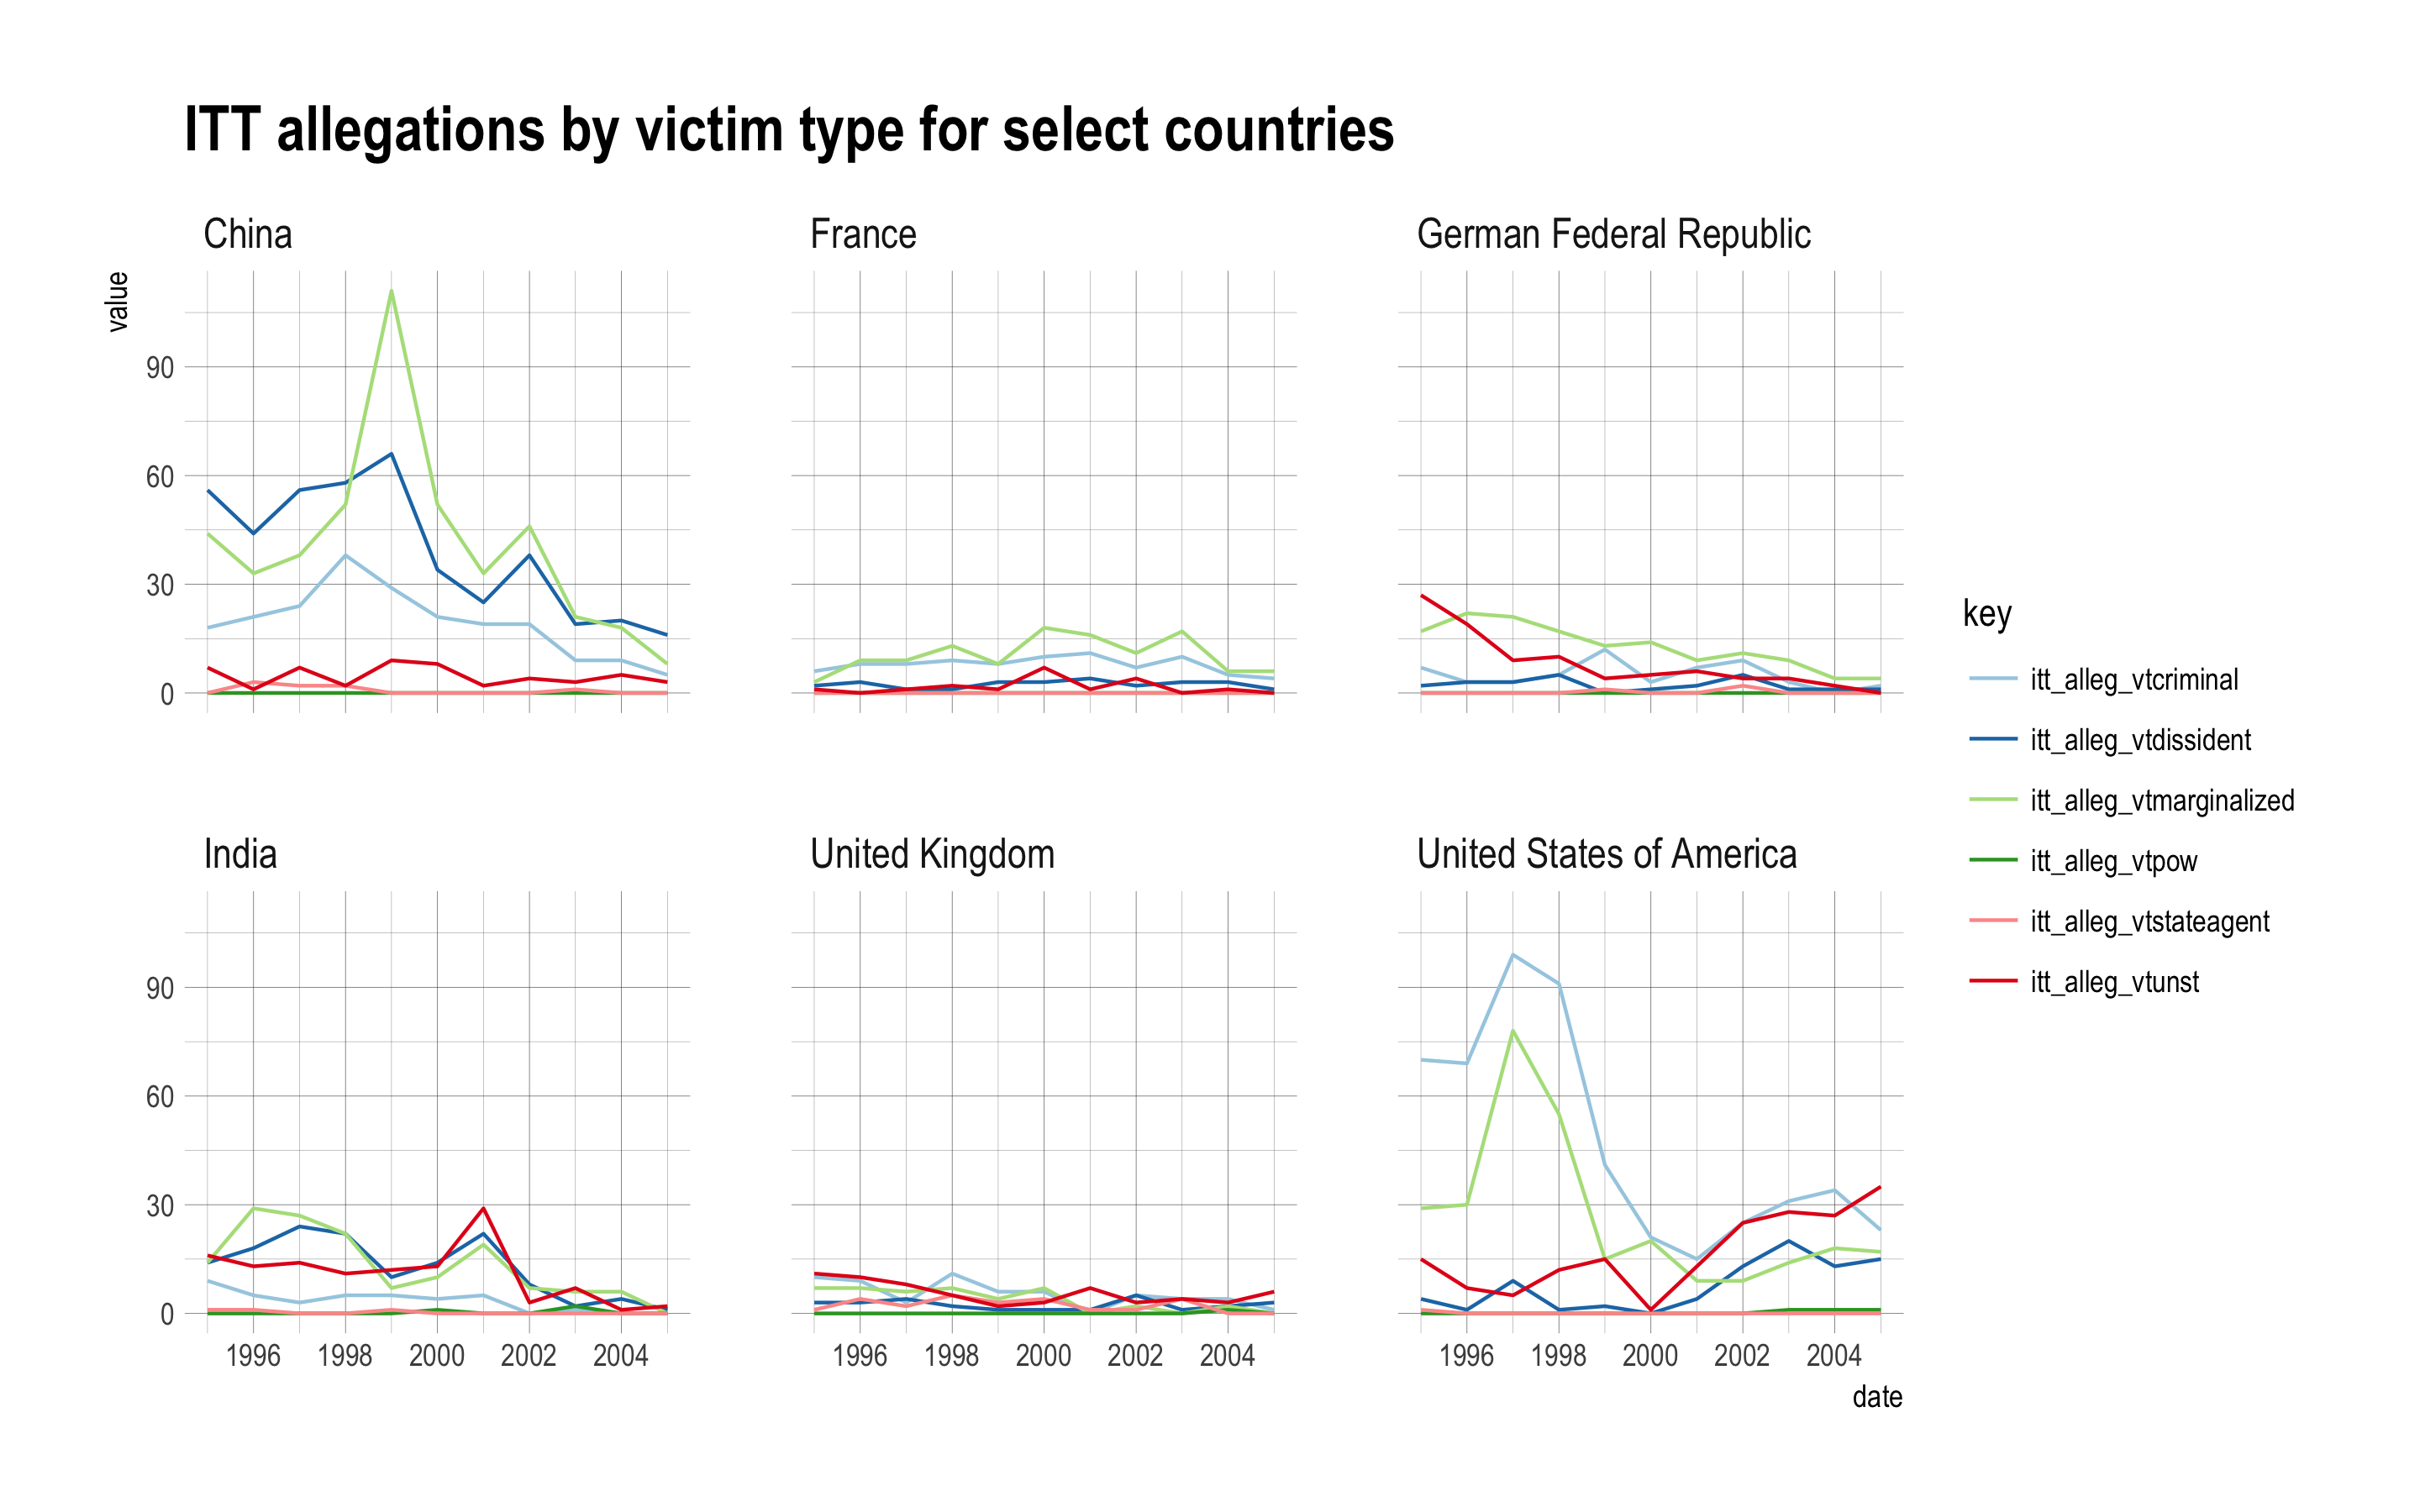
\includegraphics[width=.99\textwidth]{../output/selected-allegation-counts.png}
\end{center}
\end{figure}

The time series plots also show that allegations within a country of abuse of different kinds of victims are not always obviously correlated. While in the US allegations of abuse of criminal and marginalized victims were high in the 90's, others were not, for example. This is a broader finding. Figure \ref{fig:correlation-matrix} contains scatterplots that plot the number of allegations of torture of one victim type against another. The second plot in the rop row for example shows dissident against criminal allegations. Each line connects the observations for a country together, and color is based on the correlation coefficient. Each plot also lists the correlation coefficient for that victim type pair when we average over countries, $\bar{r}$. These correlations, if we exclude the trivial self-correlations in the diagonal, are fairly close to the global average of .34. So it is not the case that countries that torture criminals are especially prone to torture marginalized groups as well, as opposed to dissidents. This is evern more pronounced at the country level. About 20\% of the non-trivial correlations are 0 or negative, i.e. countries that have allegations of torture of one kind of victim are less likely to have allegations of torture of another kind of victim. The general point is that allegations of torturing different kinds of victims are only losely related, or, in other words, not all countries (allegedly) torture and those that do often don't (allegedly) torture the same kinds of victims. 

\begin{figure}
\begin{center}
\caption{}
\label{fig:correlation-matrix}
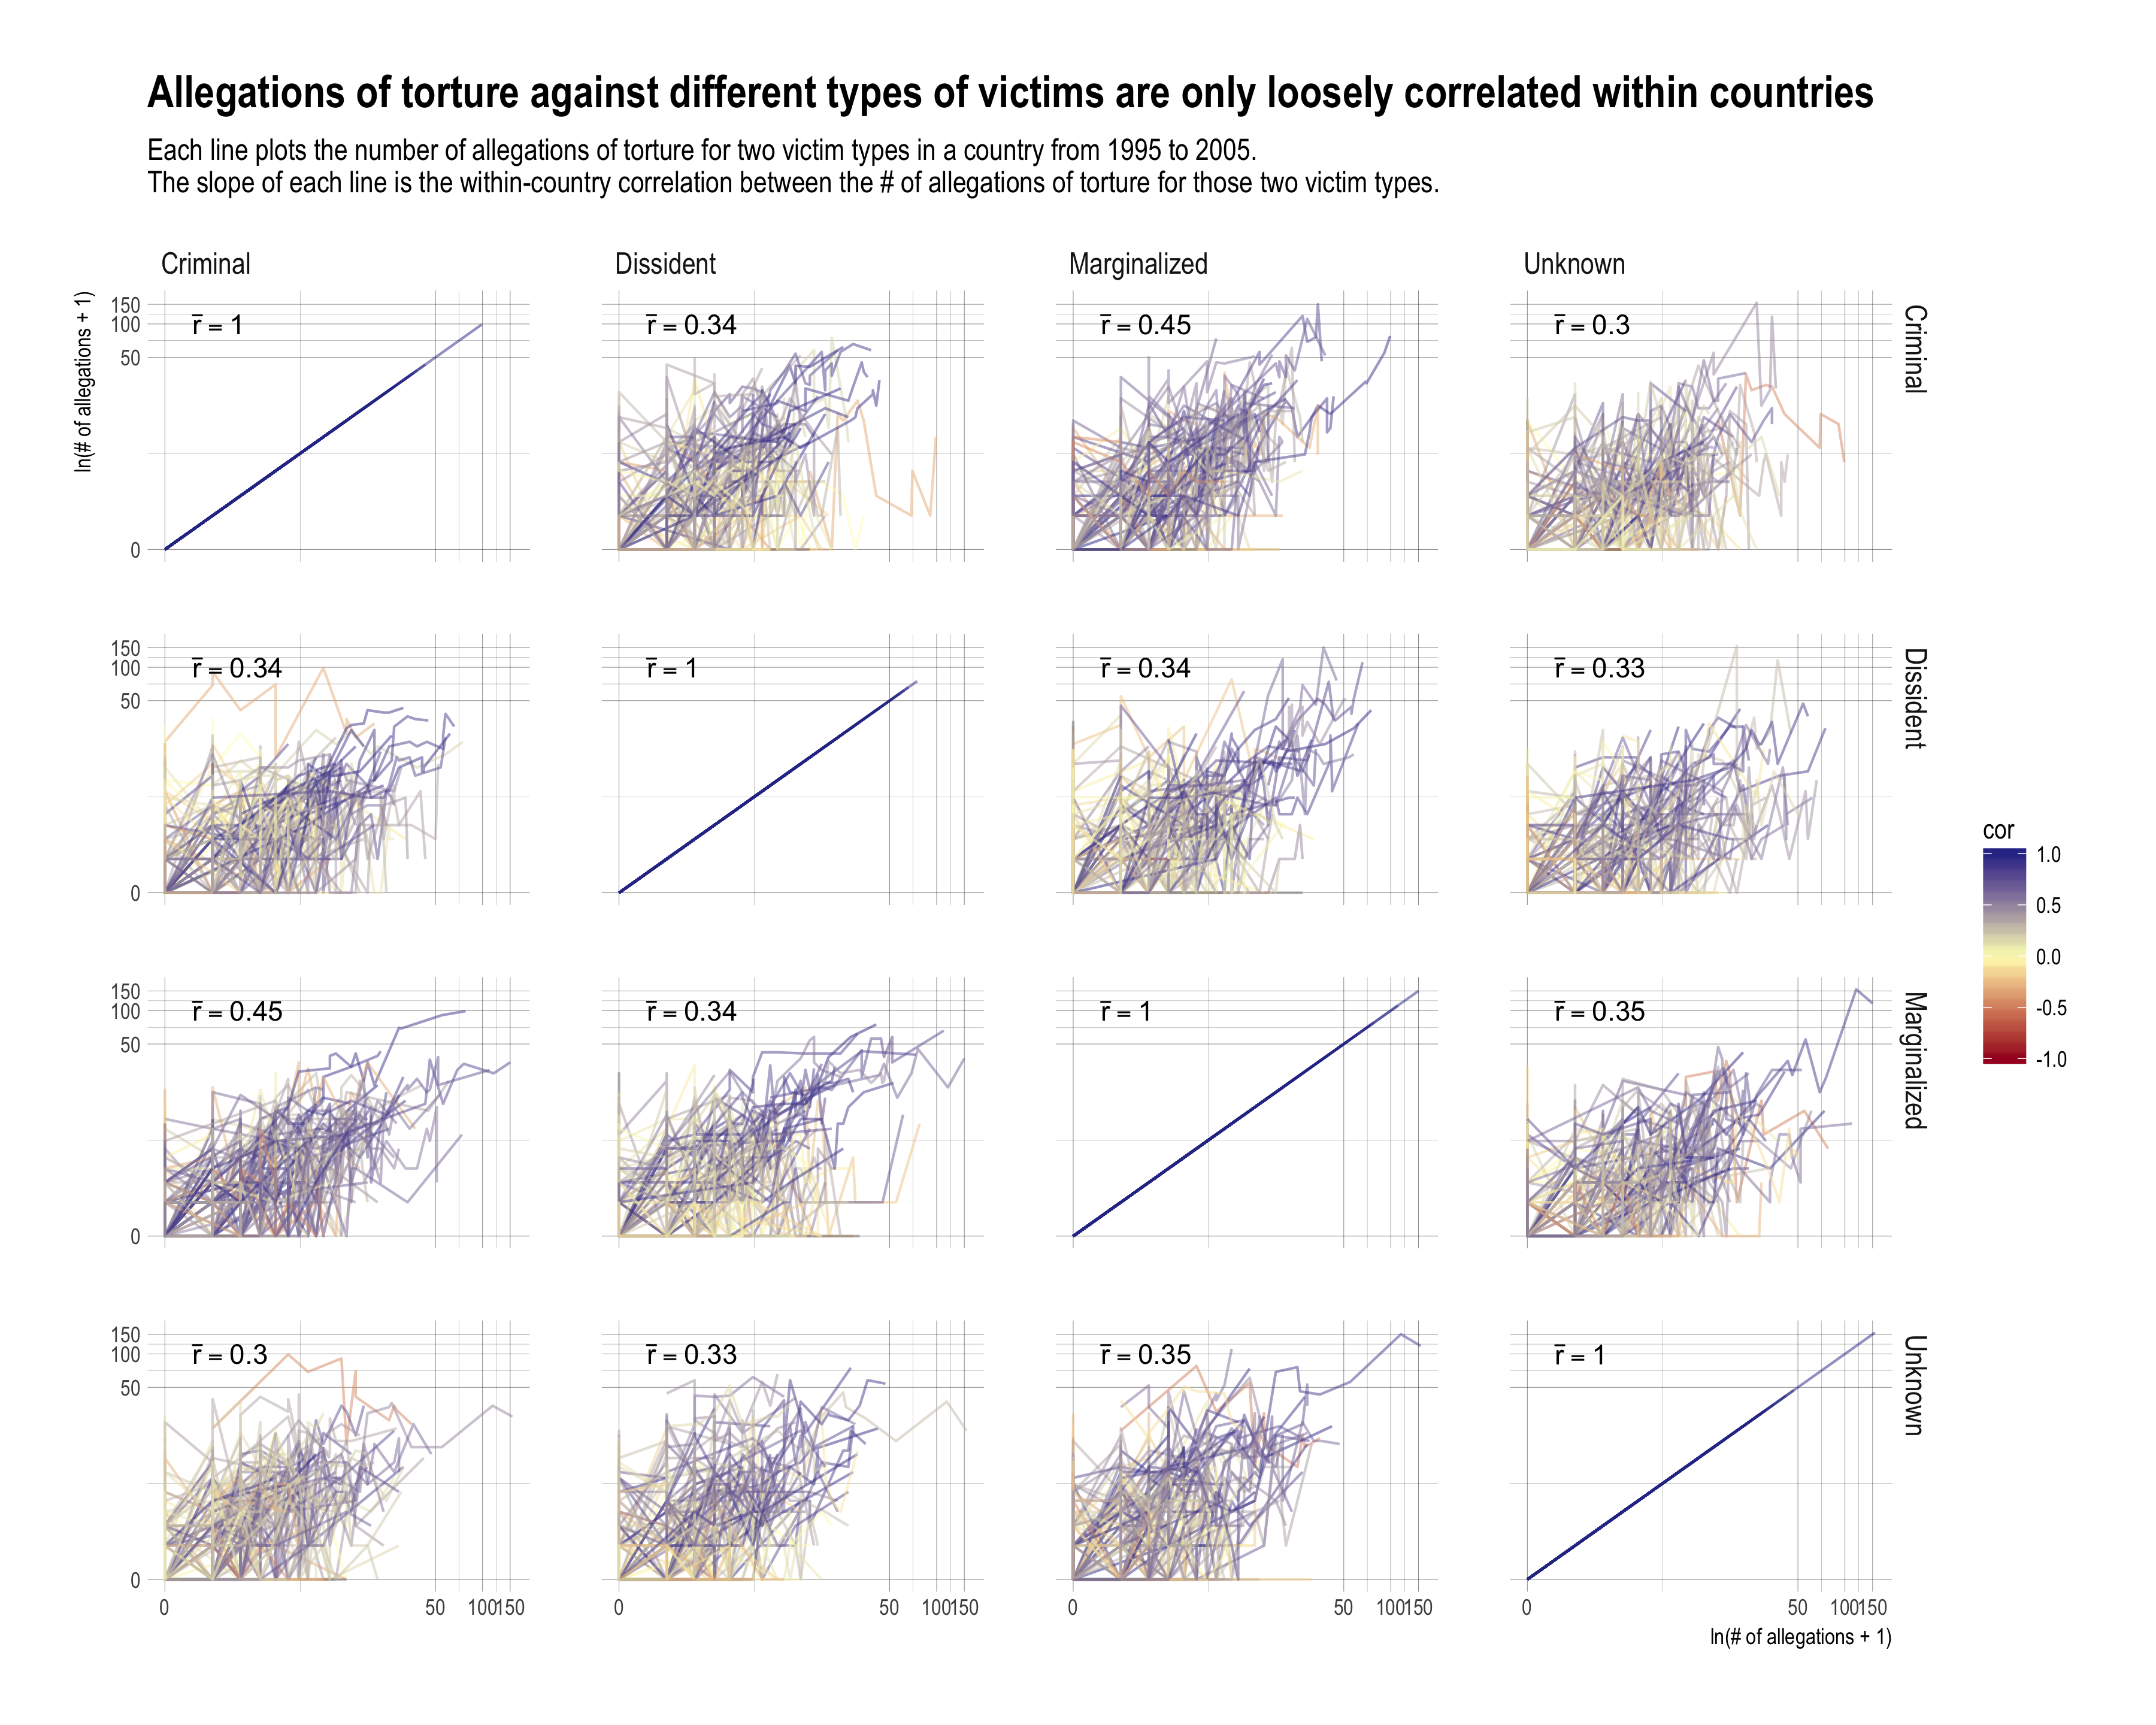
\includegraphics[width=.99\textwidth]{../output/allegations-by-victim-scatterplots.png}
\end{center}
\end{figure}

Examining that variation of allegations that a country tortures one kind of victim but not others is part of the goal of this paper. Can legal and constitutional characteristics explain why some states torture dissidents more than criminals or marginalized groups, and vice versa?

We will model three dependent variables consisting of the number of allegations against one of three victim types--criminal, marginalized, and dissident--in a given country-year. These are the three most common victim types. Our modeling strategy is to evaluate the assocation between those potentially protective factors and allegation counts separately for criminals, marginalized, and dissidents. Our results are drawn both from simple bivariate assocations and multivariate models. 

For independent and control variables, we use latent judicial independence estimates from \citet{linzer2015global}; legal system types from \citet{mitchell2013domestic}; several variables from the World Development Indicators, including GDP, population, percent of GDP from rents; and democracy indicators from V-Dem\footnote{\url{https://www.v-dem.net/en/}} and \citet{cheibub2010democracy}. A future version of this paper will also use the Comparative Constitutions Project for data on relevant constitutional provisions. 

Altogether we present results from four multivariate models. These are Poisson regression models with random intercepts for countries. We include random intercepts for two reasons. The first is that we will evaluate our models in part by their ability to predict outcomes, i.e. model fit, and including random country intercepts improves model fit a lot. The second is that by soaking up between country variation in outcomes, we can be more certain that any assocations we find for factors of interest are not spurious correlations driven by other differences between countries. The downsides are also twofold. The number of observations per group are not very large, 11 years per country at most, which could be problematic both for estimating model parameters and overfitting. The former seems to be more of an issue than the latter, as out of sample accuracy is fairly close to in-sample accuracy. And to the extent that judicial independence and legal system types really do account for cross-country differences in torture allegation levels, we are stacking the odds against finding so. 

In addition to the coefficient estimates for the variables that interest us, we also consider the impact of adding a variable on model fit, and out of sample fit specifically. This indicates how well any empirical results are to generalize outside the 11-year coverage of the data. To derive out of sample predictiosn we used 11-fold cross-validation, which roughly corresponds to predicting one year of outcomes with the remaining 10 years of data. 

Figures \ref{fig:coefs} and \ref{fig:fit} show the coefficient estimates and model fit for the 6 models we estimated in total. The first model is an intercept only model, i.e. with the global and country random intercepts, and establishes one of the baselines for fit. The last model is a commonly used machine learning predictive model, XGBoost, which provides another benchmark of the levels of prediction accuracy one should expect to be feasible. The model is an ensemble of decision trees, where each decision tree is specifically trained to reduce leftover prediction error given the current ensemble prediction. Each component decision tree itself is a very simple model that predicts allegation counts by splitting the input data into several groups based on the values observations have on selected independent variables. Hyperparameters for this kind of model are usually tuned via cross-validation. In order to be able to compare the cross-validation predictions to those from the count models, we did not do this and instead left hyperparameters at their default values.

\begin{figure}
\begin{center}
\caption{Coefficient estimates for Poisson regression models of torture allegation counts by victim type. All models include random country intercepts.}
\label{fig:coefs}
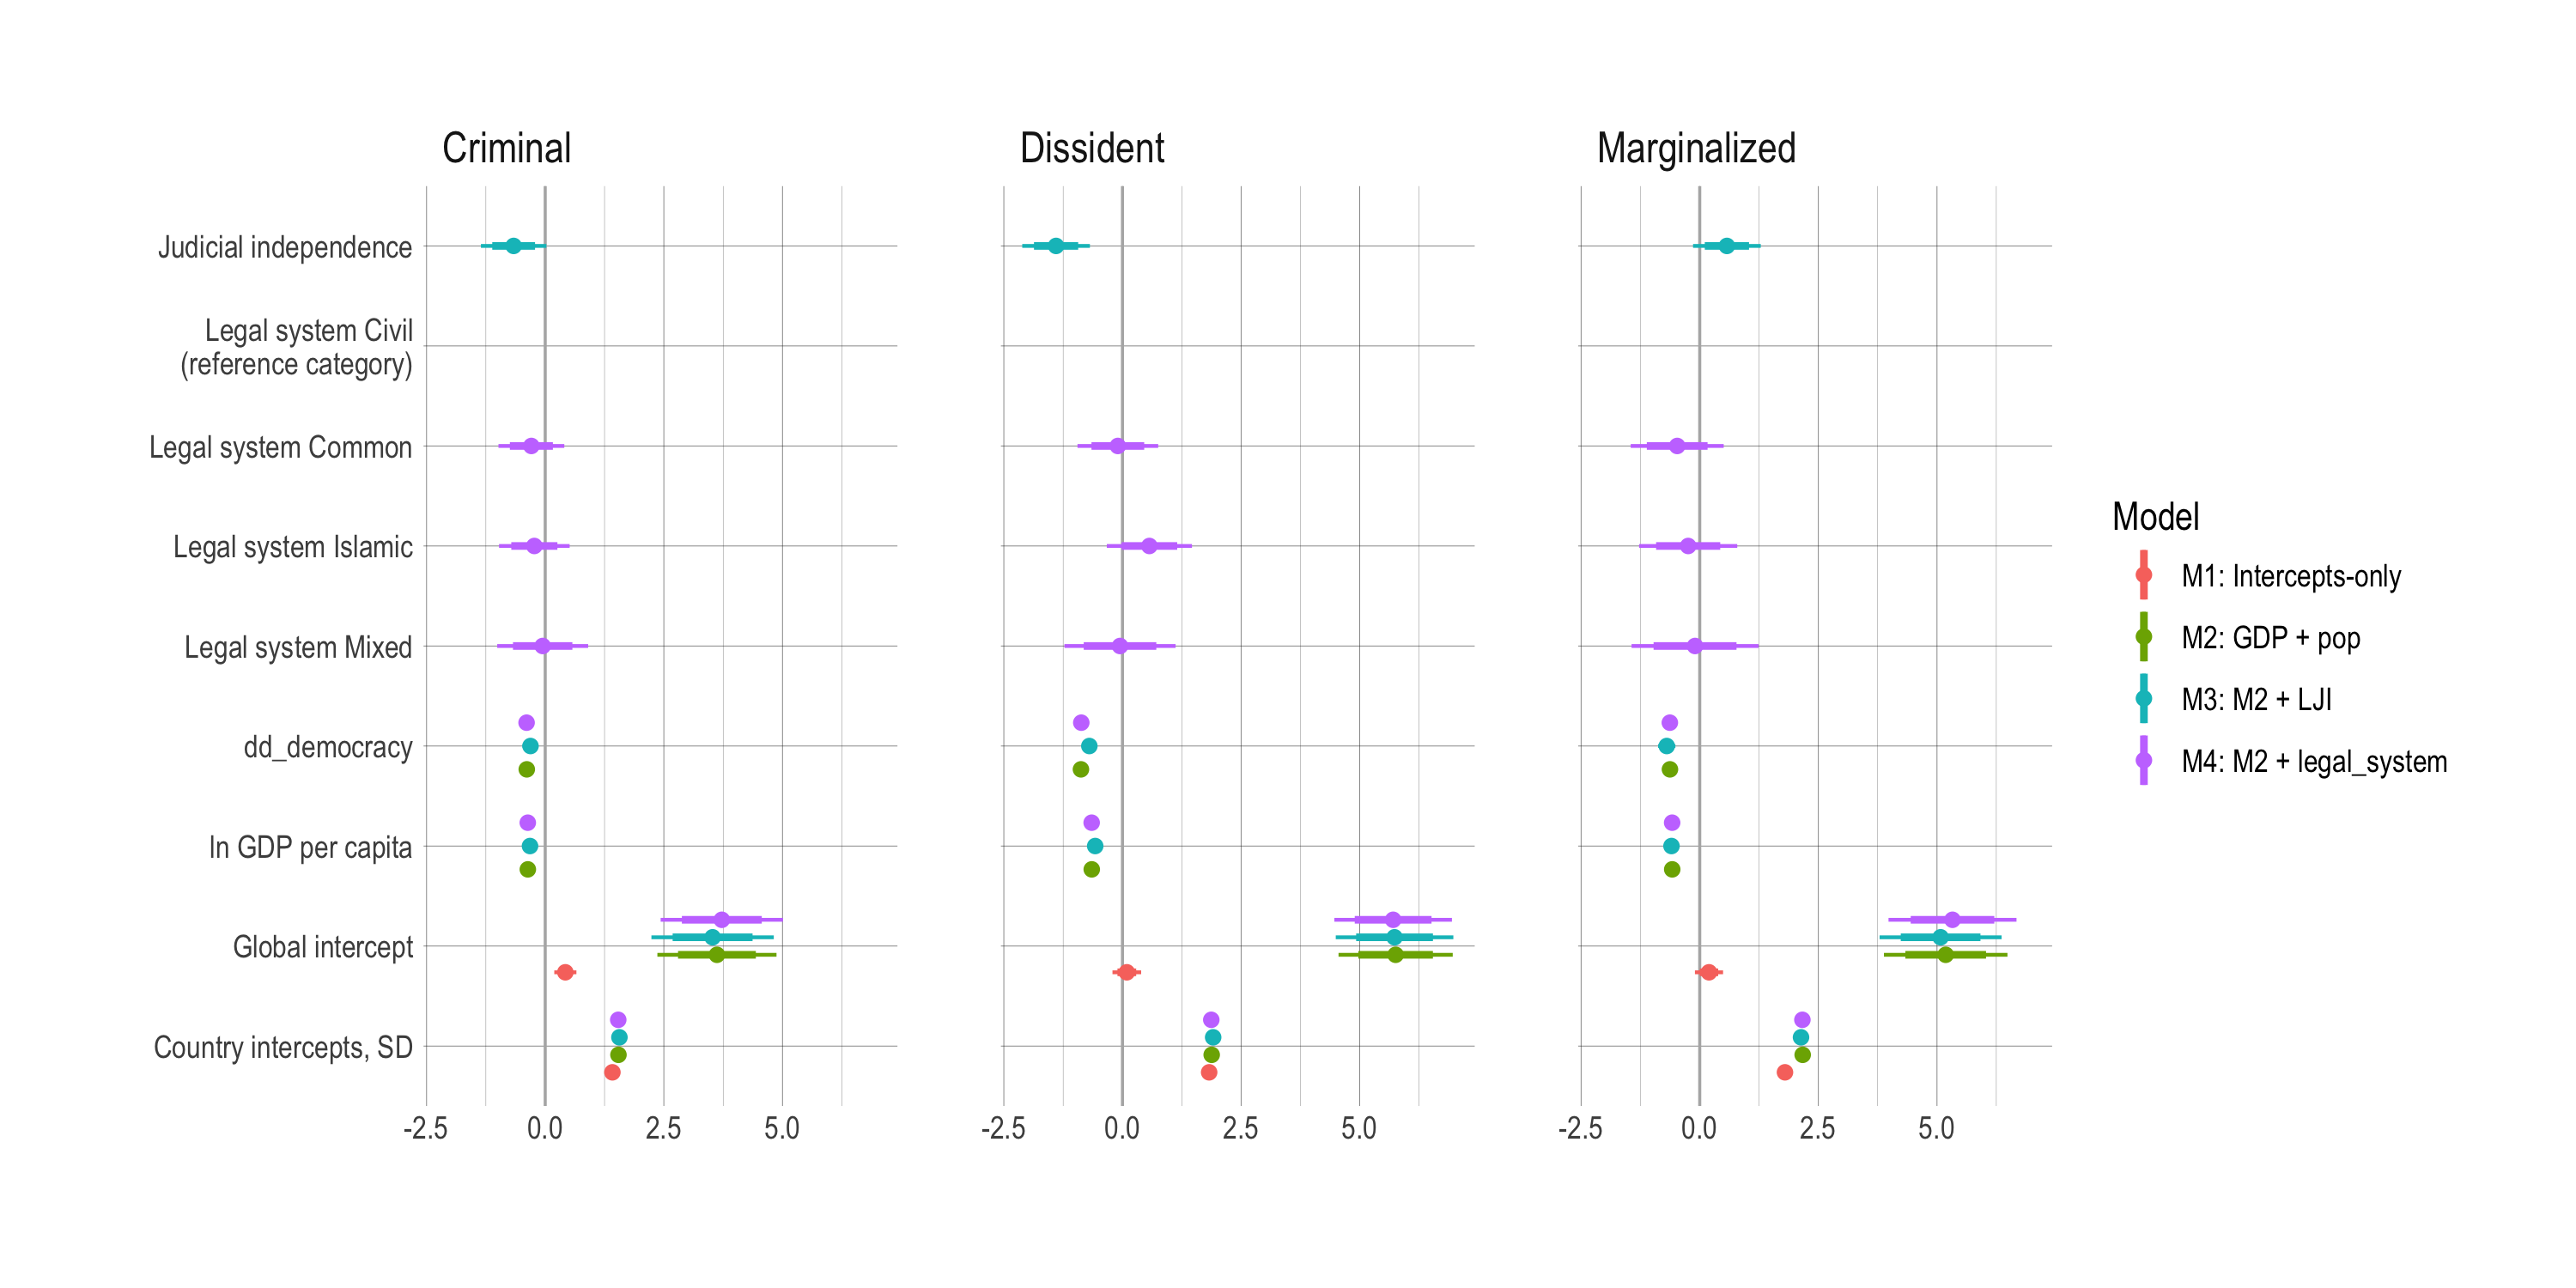
\includegraphics[width=.99\textwidth]{../output/count-model-coefs.png}
\end{center}
\end{figure}

\begin{figure}
\begin{center}
\caption{Model fit and predictive accuracy. Mean absolute error (MAE) and root mean squared error (RMSE) are calculated using out of sample predictions obtained via 11-fold cross-validation.}
\label{fig:fit}
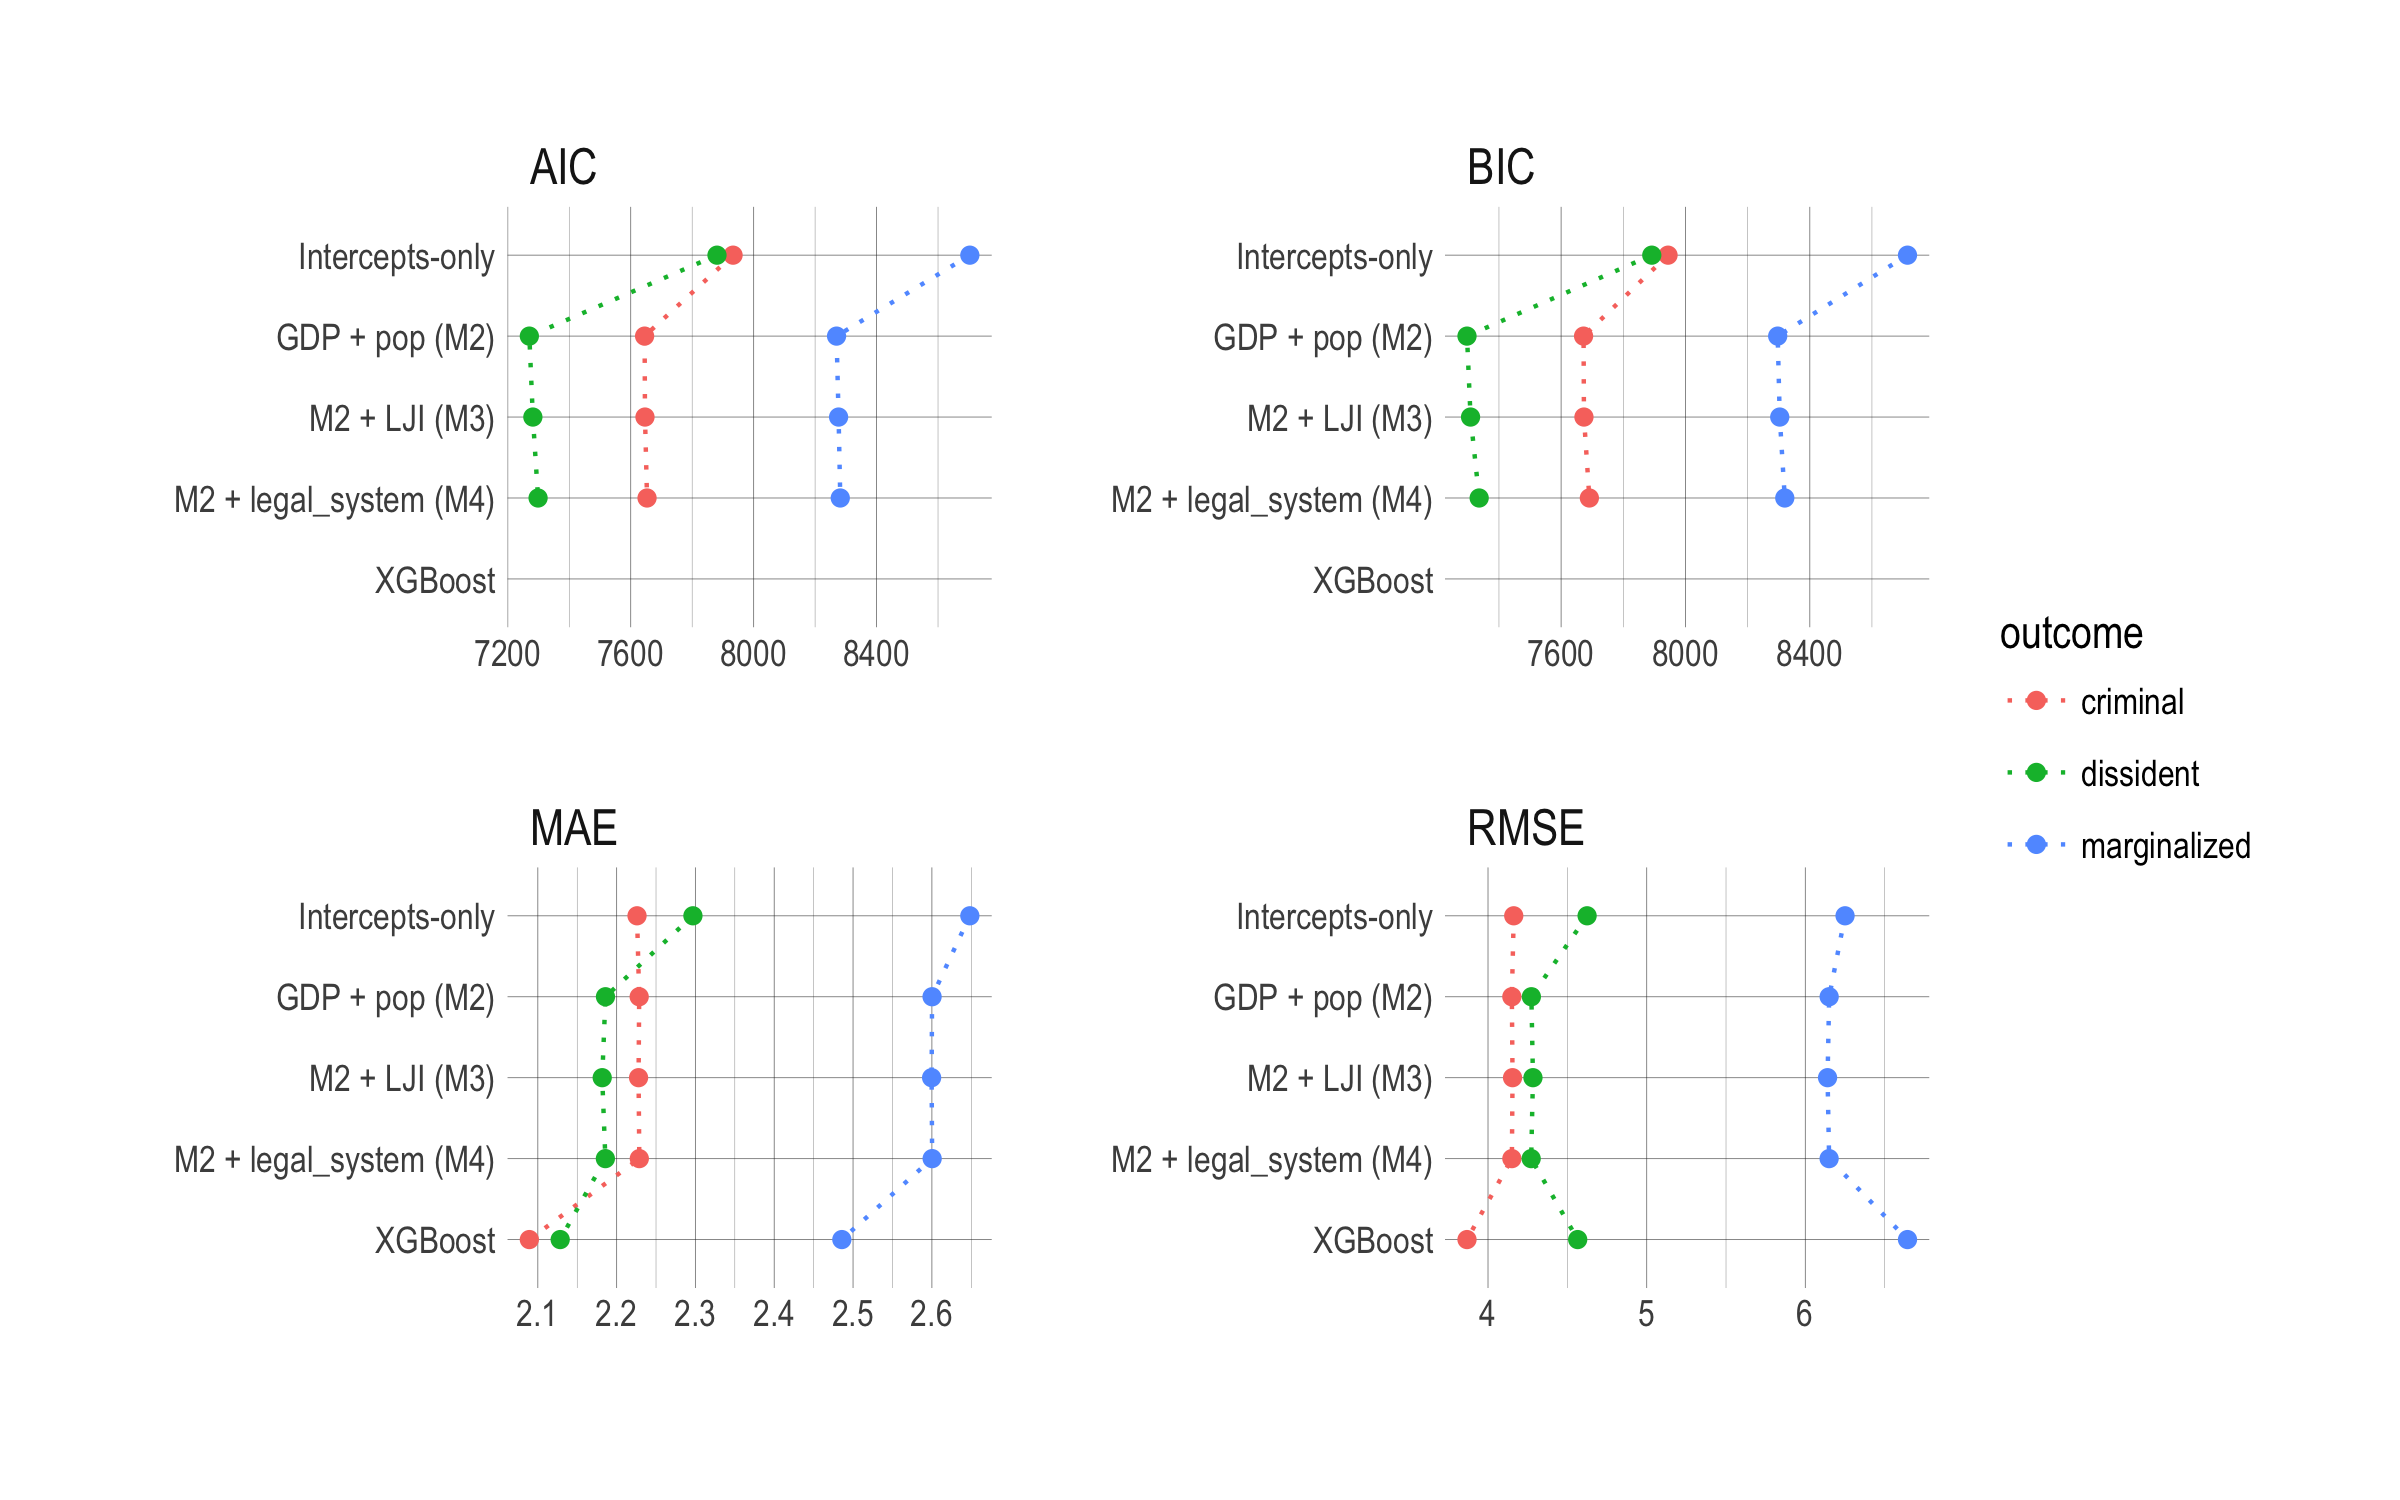
\includegraphics[width=.99\textwidth]{../output/model-fit-plot.png}
\end{center}
\end{figure}

\begin{figure}
\begin{center}
\caption{Predicted versus observed values for the country intercepts-only model (model 1), as an example of what the predictions for all models look like.}
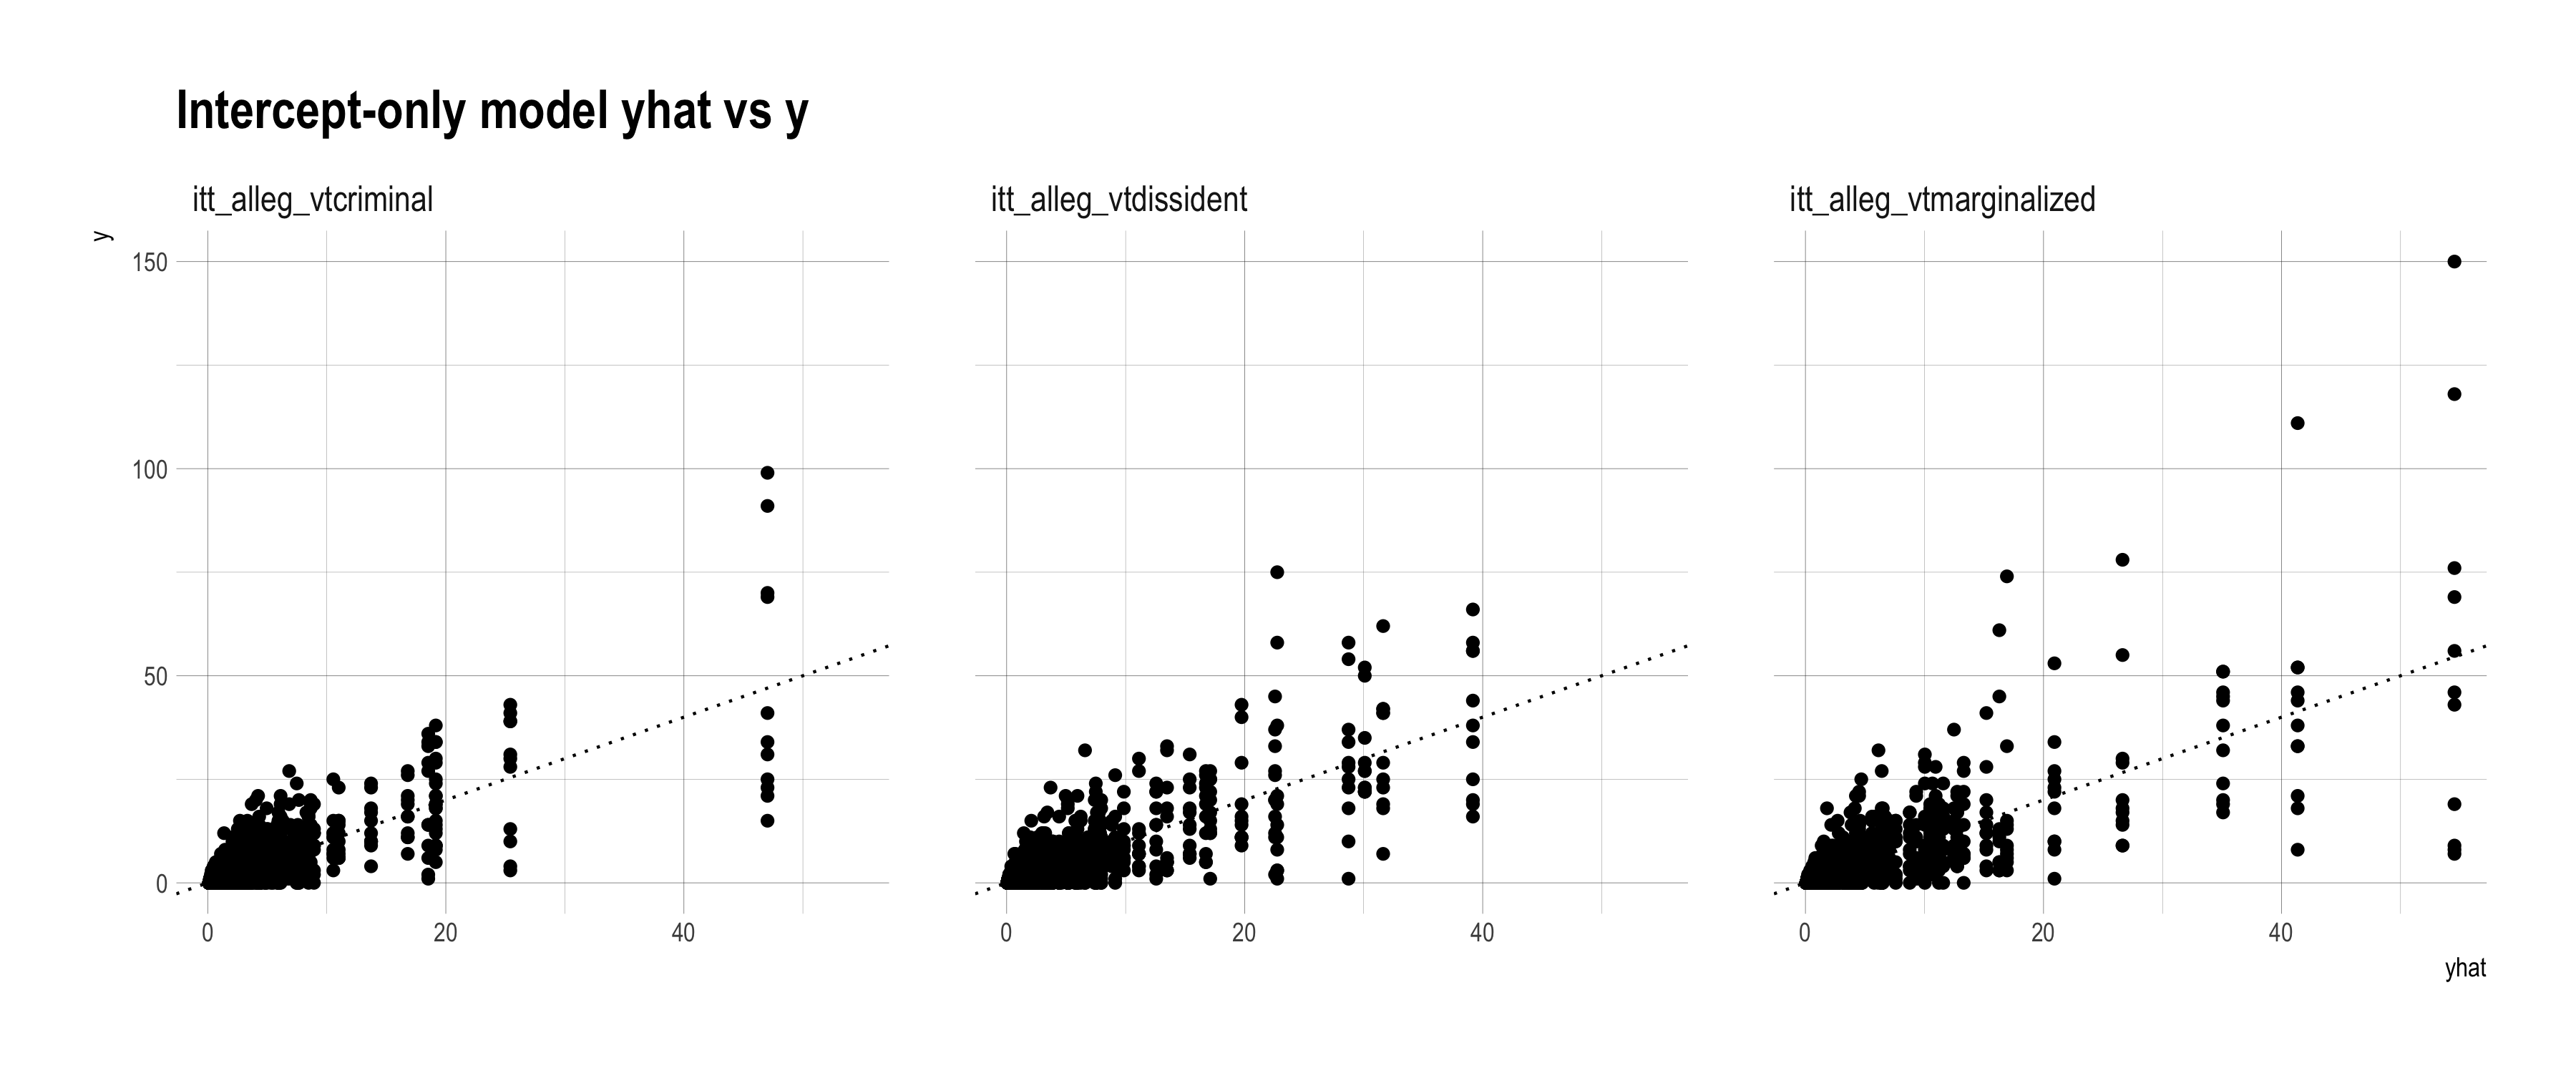
\includegraphics[width=.99\textwidth]{../output/mdl1-y-vs-yhat.png}
\end{center}
\end{figure}

The second count model adds GDP per capita and a binary democracy indicator. These are retained as control variables in the subsequent models. The binary democracy indicator is derived from the Cheibub et al democracy data. This codes six types of regimes, three each for democracies and dictatorships. We collapse the subtypes into a single binary democracy/dictatorship indicator. Adding these two variables significantly improves fit accross all metrics we consider in Figure \ref{fig:fit}.

\textbf{Judicial independence}. The first factor we examine estimates of latent judicial independence, a continuous variable ranging from 0 to 1. Bivariate plots of judicial independence in Figure \ref{fig:lji-bivariate} show that it is related with a decrease in allegations of dissident torture, but it is also apparent that the effect size is not very large in relation to the overall variation in allegation counts. The blue lines show fitted regression lines, and for dissident allegations the coefficient is negative and statistically significant with $p<0.05$. 

Judicial independence is strongly related to regime type, being higher in democracies than dictatorships in general, and highest in parliamentary democracies specifically. In model three, we estimate the effect of judicial independence when controlling for democracy, and the effect on dissident torture remains negative and significant. Judicial independence is associated with a reduced number of dissdent torture allegations, in addition to any protective effects provided in democracies generally. 

In terms of model fit however, adding judicial indepencence does not clearly improve predictive accuracy. The MAE and RMSE slightly decrease, but not by enough to justify the added model complexity if we look at the information criteria AIC and BIC. 

One potential saving grace is provided by the XGBoost model results. It is common to evaluate the input variables for a machine learning model by how much they effect the model's predictive accuracy--"variable importance", and these numbers are shown in Figure \ref{var-imp}. The higher the variable importance, the more a variable matters for predicting the outcome, and latent judicial independence ("LJI") is fairly high up by average importance accross the three outcomes, fifth after GDP, country population, \% of GDP from rents, and GDP per capita. 

Since the XGBoost model does not include random country intercepts and thus reflects a variable's ability to predict between country differences more than the count models with random intercepts do, we can tentatively conclude that the model fit tells us that (1) increases in judicial independence appear to be related to a decrease in torture allegations of dissidents, but (2) also that judicial independence has a stronger ability to explain between country differences in torture allegations. 

\textbf{Democracy}. Democracy itself, if we look at the estimates accross all models and outcomes, appears to be robustly related to a decrease in torture allegations against victims of all three kinds. That probably matches prior expectations, but also is a finding that appears simpler than it is. The relationship betwen democracy and torture allegations estimated in the model are conditional on country wealth and average levels of allegations in a country, via the random intercept. With judicial independence, it turned out that the multivariate effect estimates matched the unconditional, bivariate findings. This is no the case with democracy. 

Unconditionally, and going by allegation numbers, democracies only torture dissidents less than dictatorships. They are accused of torturing marginalized and criminal victims as much or even more than dictatorships are. Figure \ref{democracy} shows the average number of allegations for each of the six regime types in the Cheibub et all classification. Only for dissident victims are the averages when we compare the three democratic and dictatorship regime sub-types clearly lower. One neccessary word of caution here is that while the averages differ, there is a lot of variation around these averages, i.e. differences between groups are outweighted by differences among individual countries and country-years. 

What do we make of this finding? As with judicial independence, they key might lie with changes over time versus differences between countries. Tentatively, it seems that countries that change to a democratic regime type experience a decrease in torture allegations against dissidents, but not criminals and marginalized victimes, and also that overall democratic countries experience higher levels of torture allegations that we might otherwise expect, for reasons that are not clear, or at least not related to wealth alone. 

We did not specifically examine the impact of including the binary democracy indicator on model fit. Probably wealth accounts for most of the fit improvement if we compare models 1 and 2, and the XGBoost results also do not bode well. Logically, the ability of a binary indicator to predict count outcomes will be limited. 

\begin{figure}
\begin{center}
\caption{Bivariate relationships between latent judicial independence and torture allegations by victim type}
\label{fig:lji-bivariate}
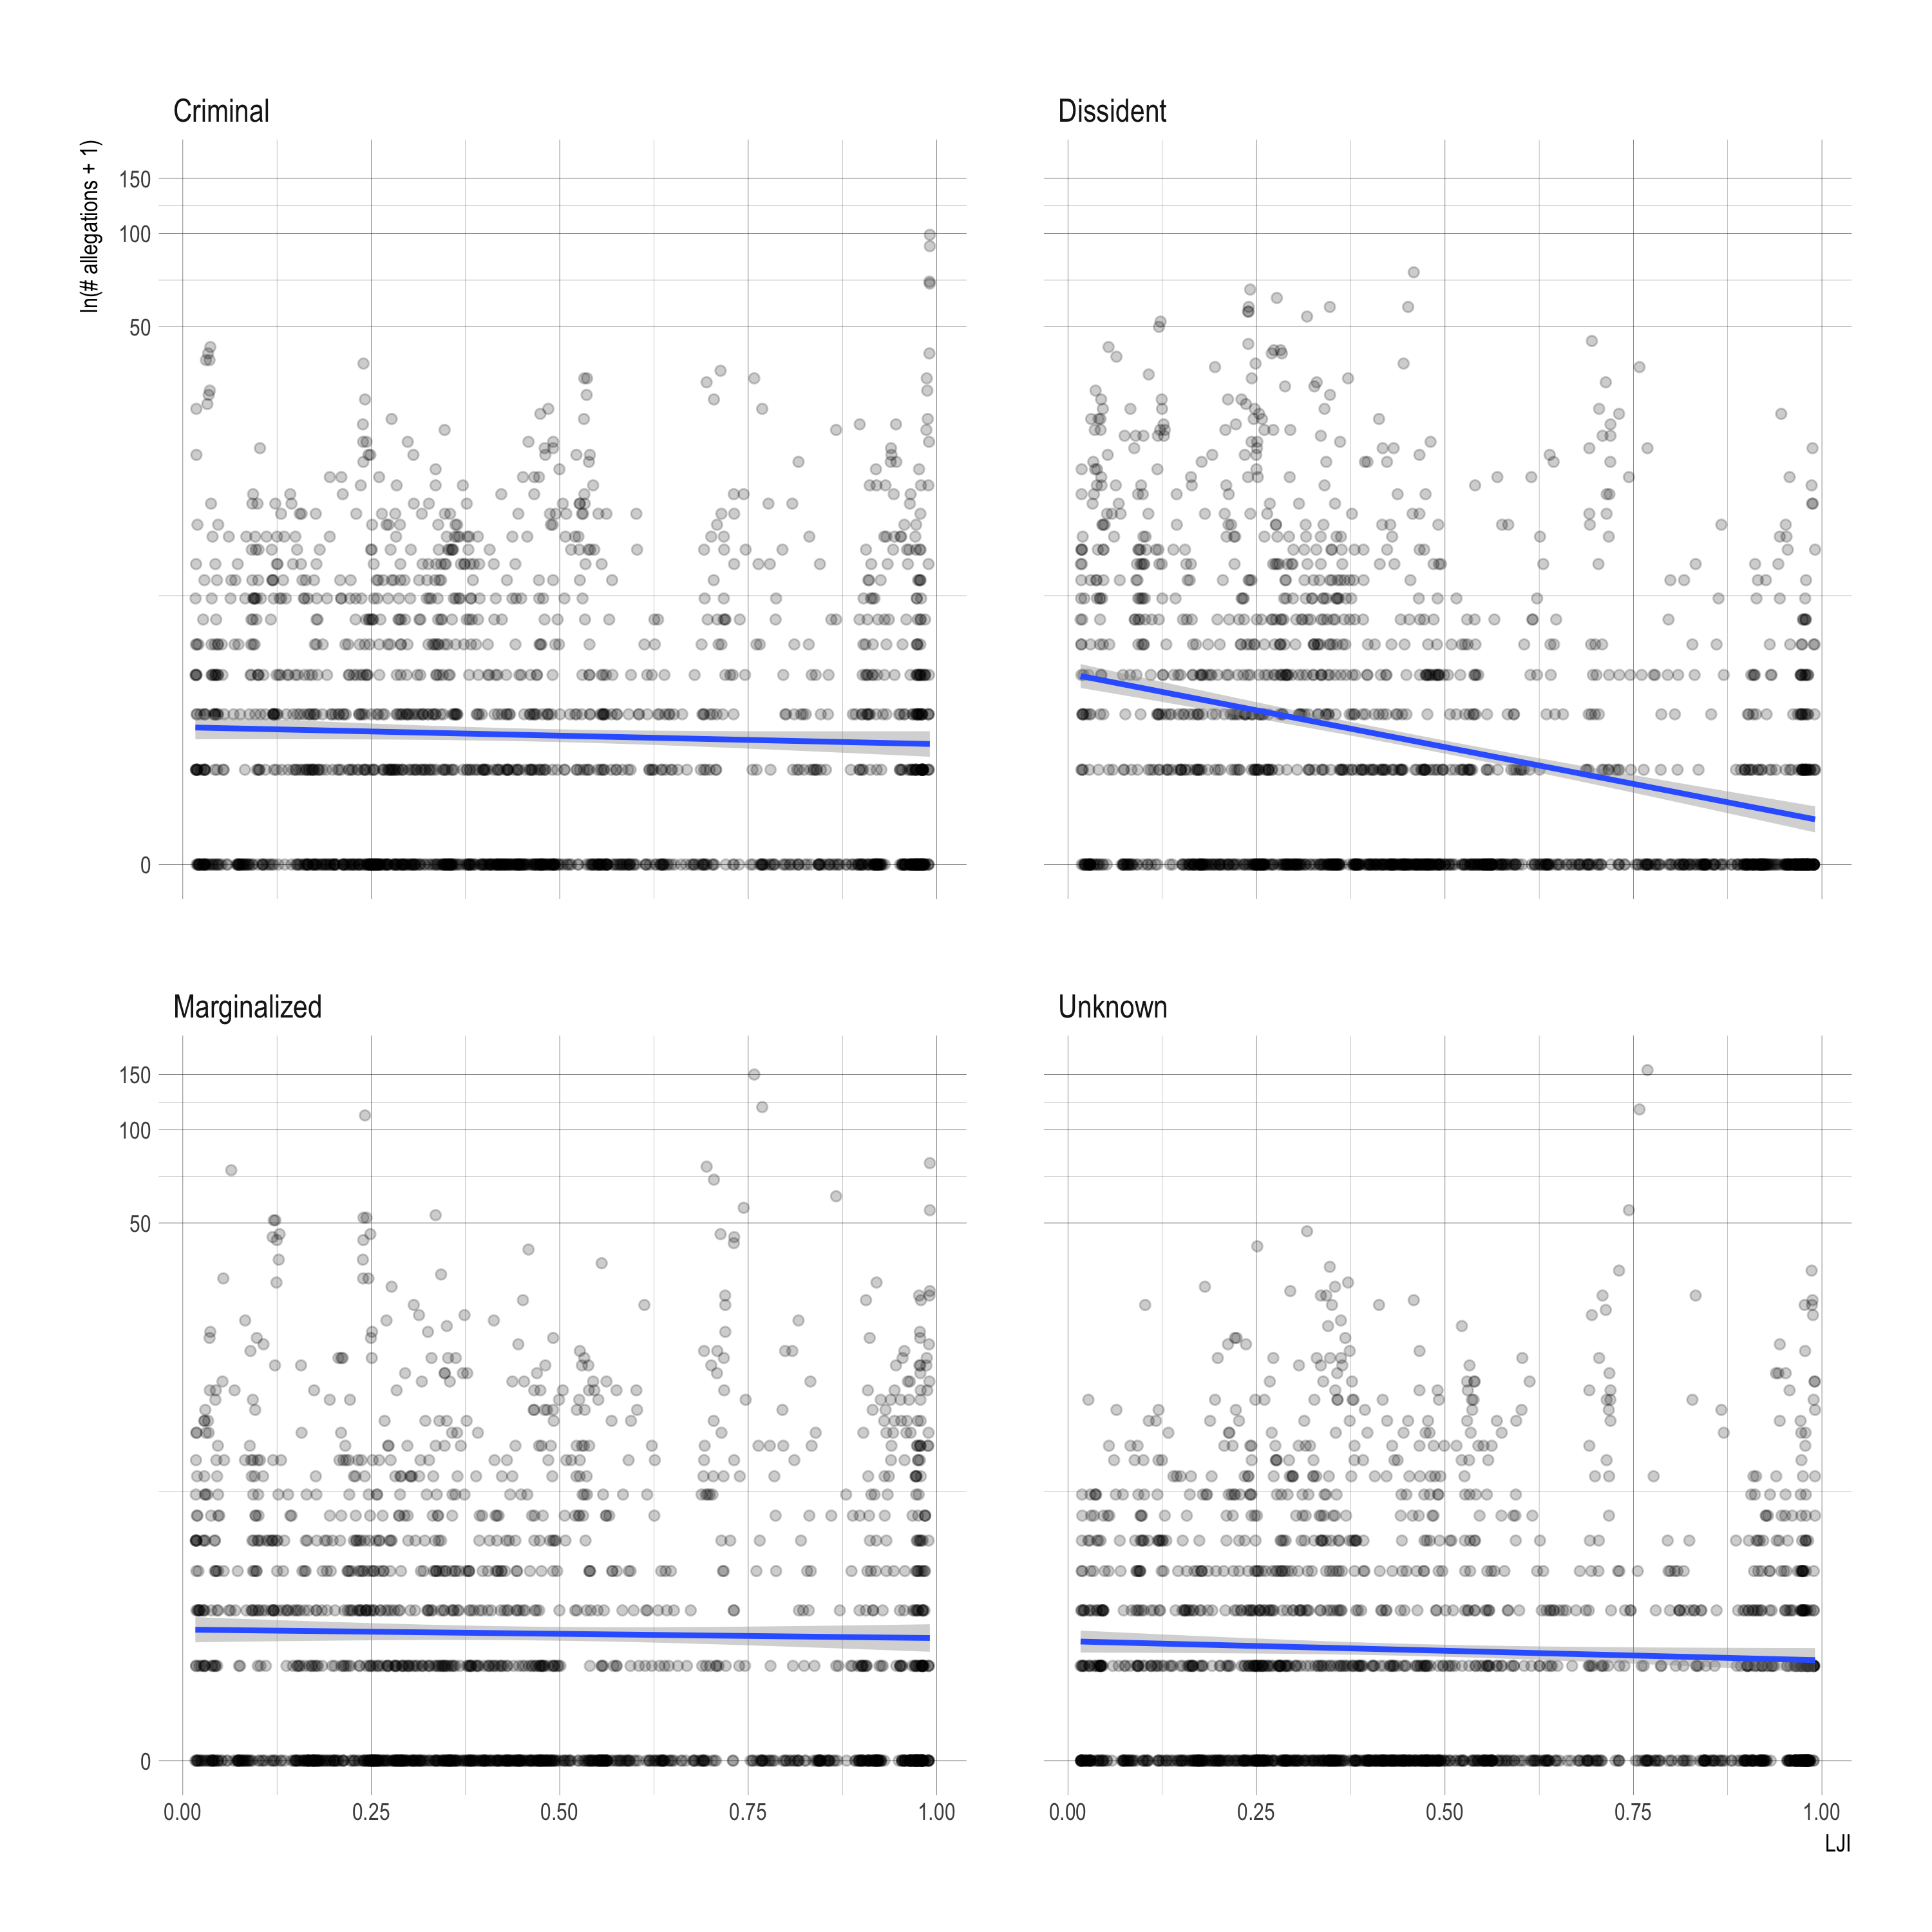
\includegraphics[width=.7\textwidth]{../output/scatterplot-itt-allegations-v-lji.png}
\end{center}
\end{figure}

\begin{figure}
\begin{center}
\caption{XGBoost variable importance for predictive accuracy.}
\label{var-imp}
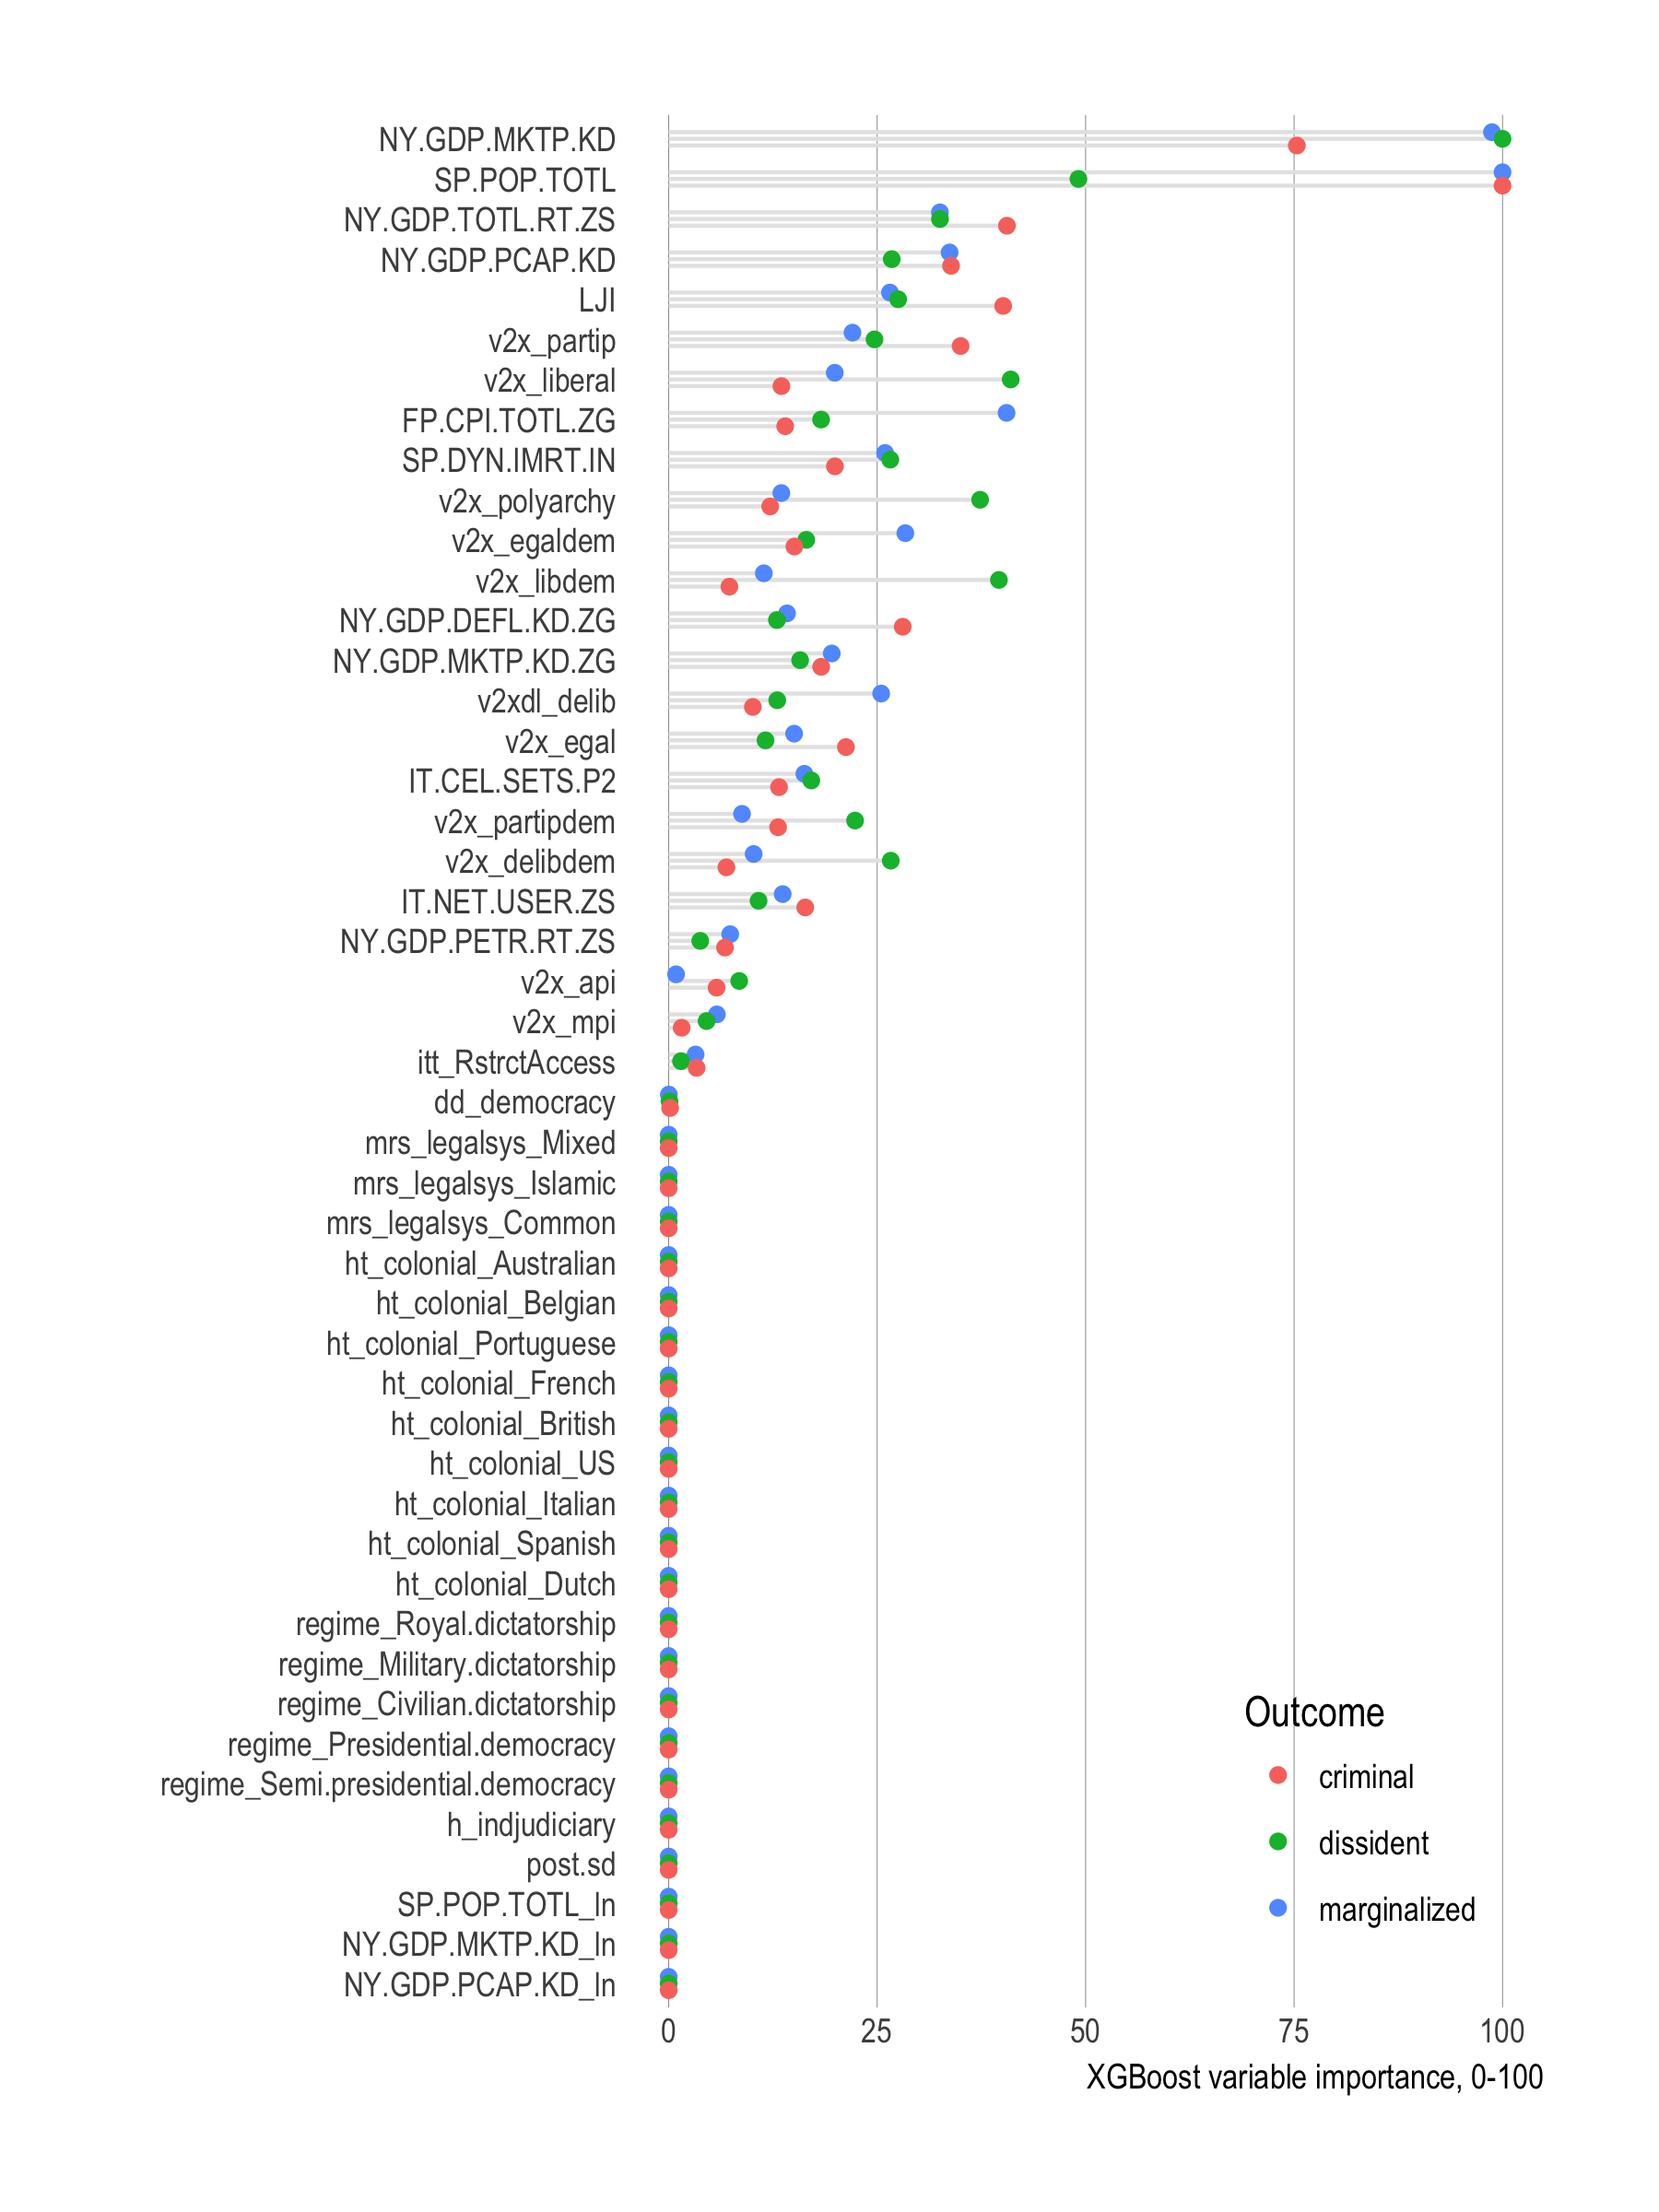
\includegraphics[width=.99\textwidth]{../output/xgboost-variable-importance.png}
\end{center}
\end{figure}

\begin{figure}
\begin{center}
\caption{Average number of torture allegations by victim type and regime type. Note that variation of cases around the averages is much larger than differences between the averages.}
\label{democracy}
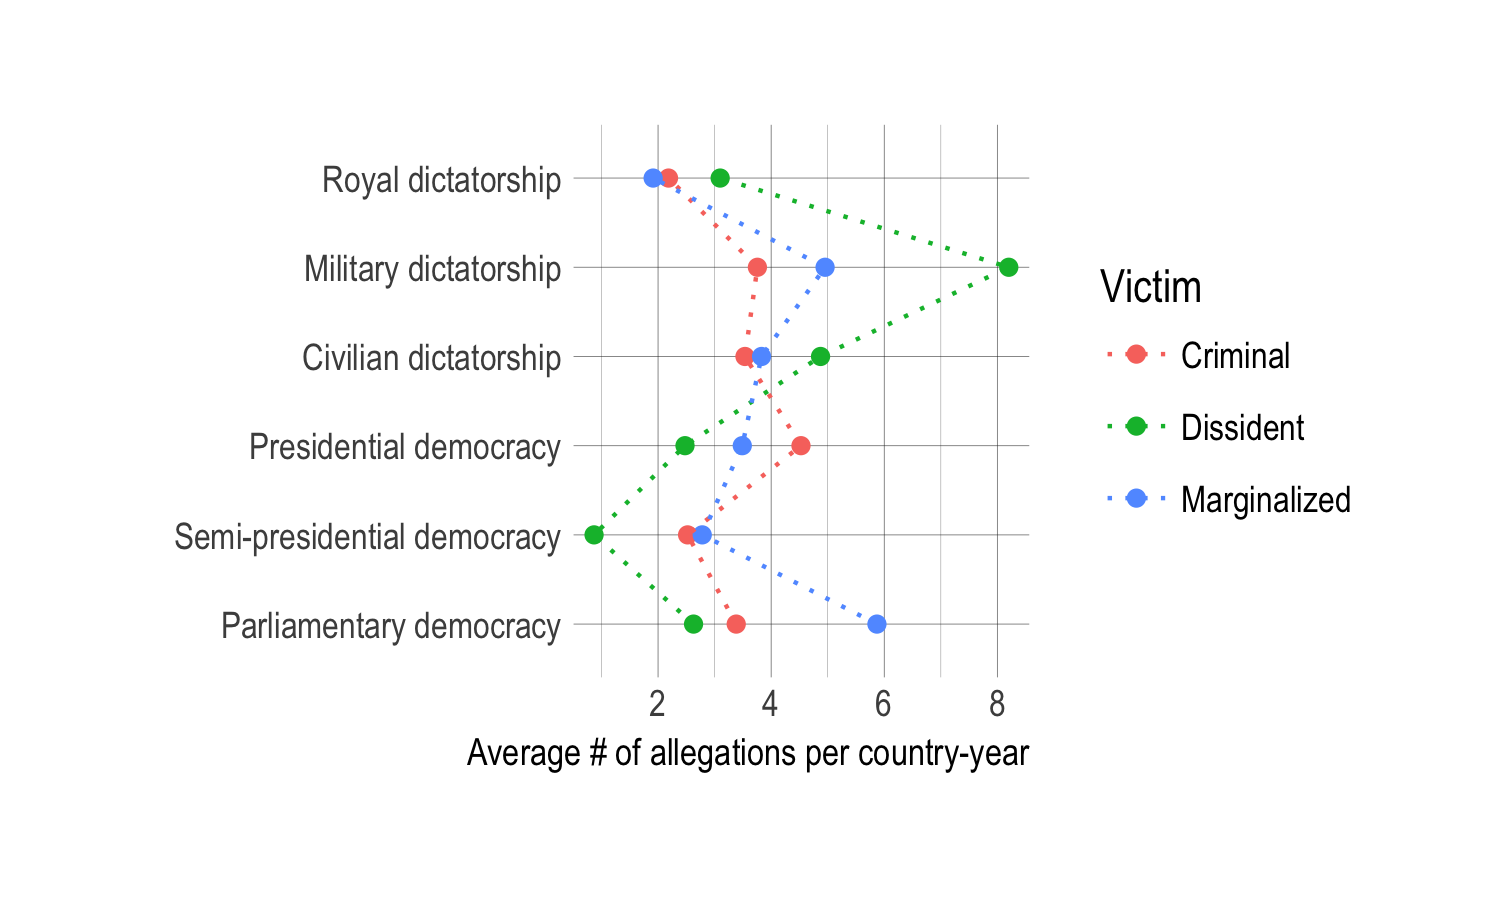
\includegraphics[width=.7\textwidth]{../output/avg-allegations-by-regime.png}
\end{center}
\end{figure}

\textbf{Legal system}. The last factor we consider is legal system type. The \citet{mitchell2013domestic} classification has four categories: civil, common law, Islamic, and mixed systems. Civil law systems are the most common and we leave this as the reference category. Although the raw data hint at a higher level of allegations of torture of dissidents, and to a lesser extent criminal, in Islamic legal systems (Figure \ref{legal-system}), these differences are not very large and disappear in the multivariate estimates in model 4 in Figure \ref{fig:coefs}. Model fit also suggests that legal system types do not have much of a relationship with torture allegations. 

\begin{figure}
\begin{center}
\caption{Torture allegations by victim type accross legal system types}
\label{legal-system}
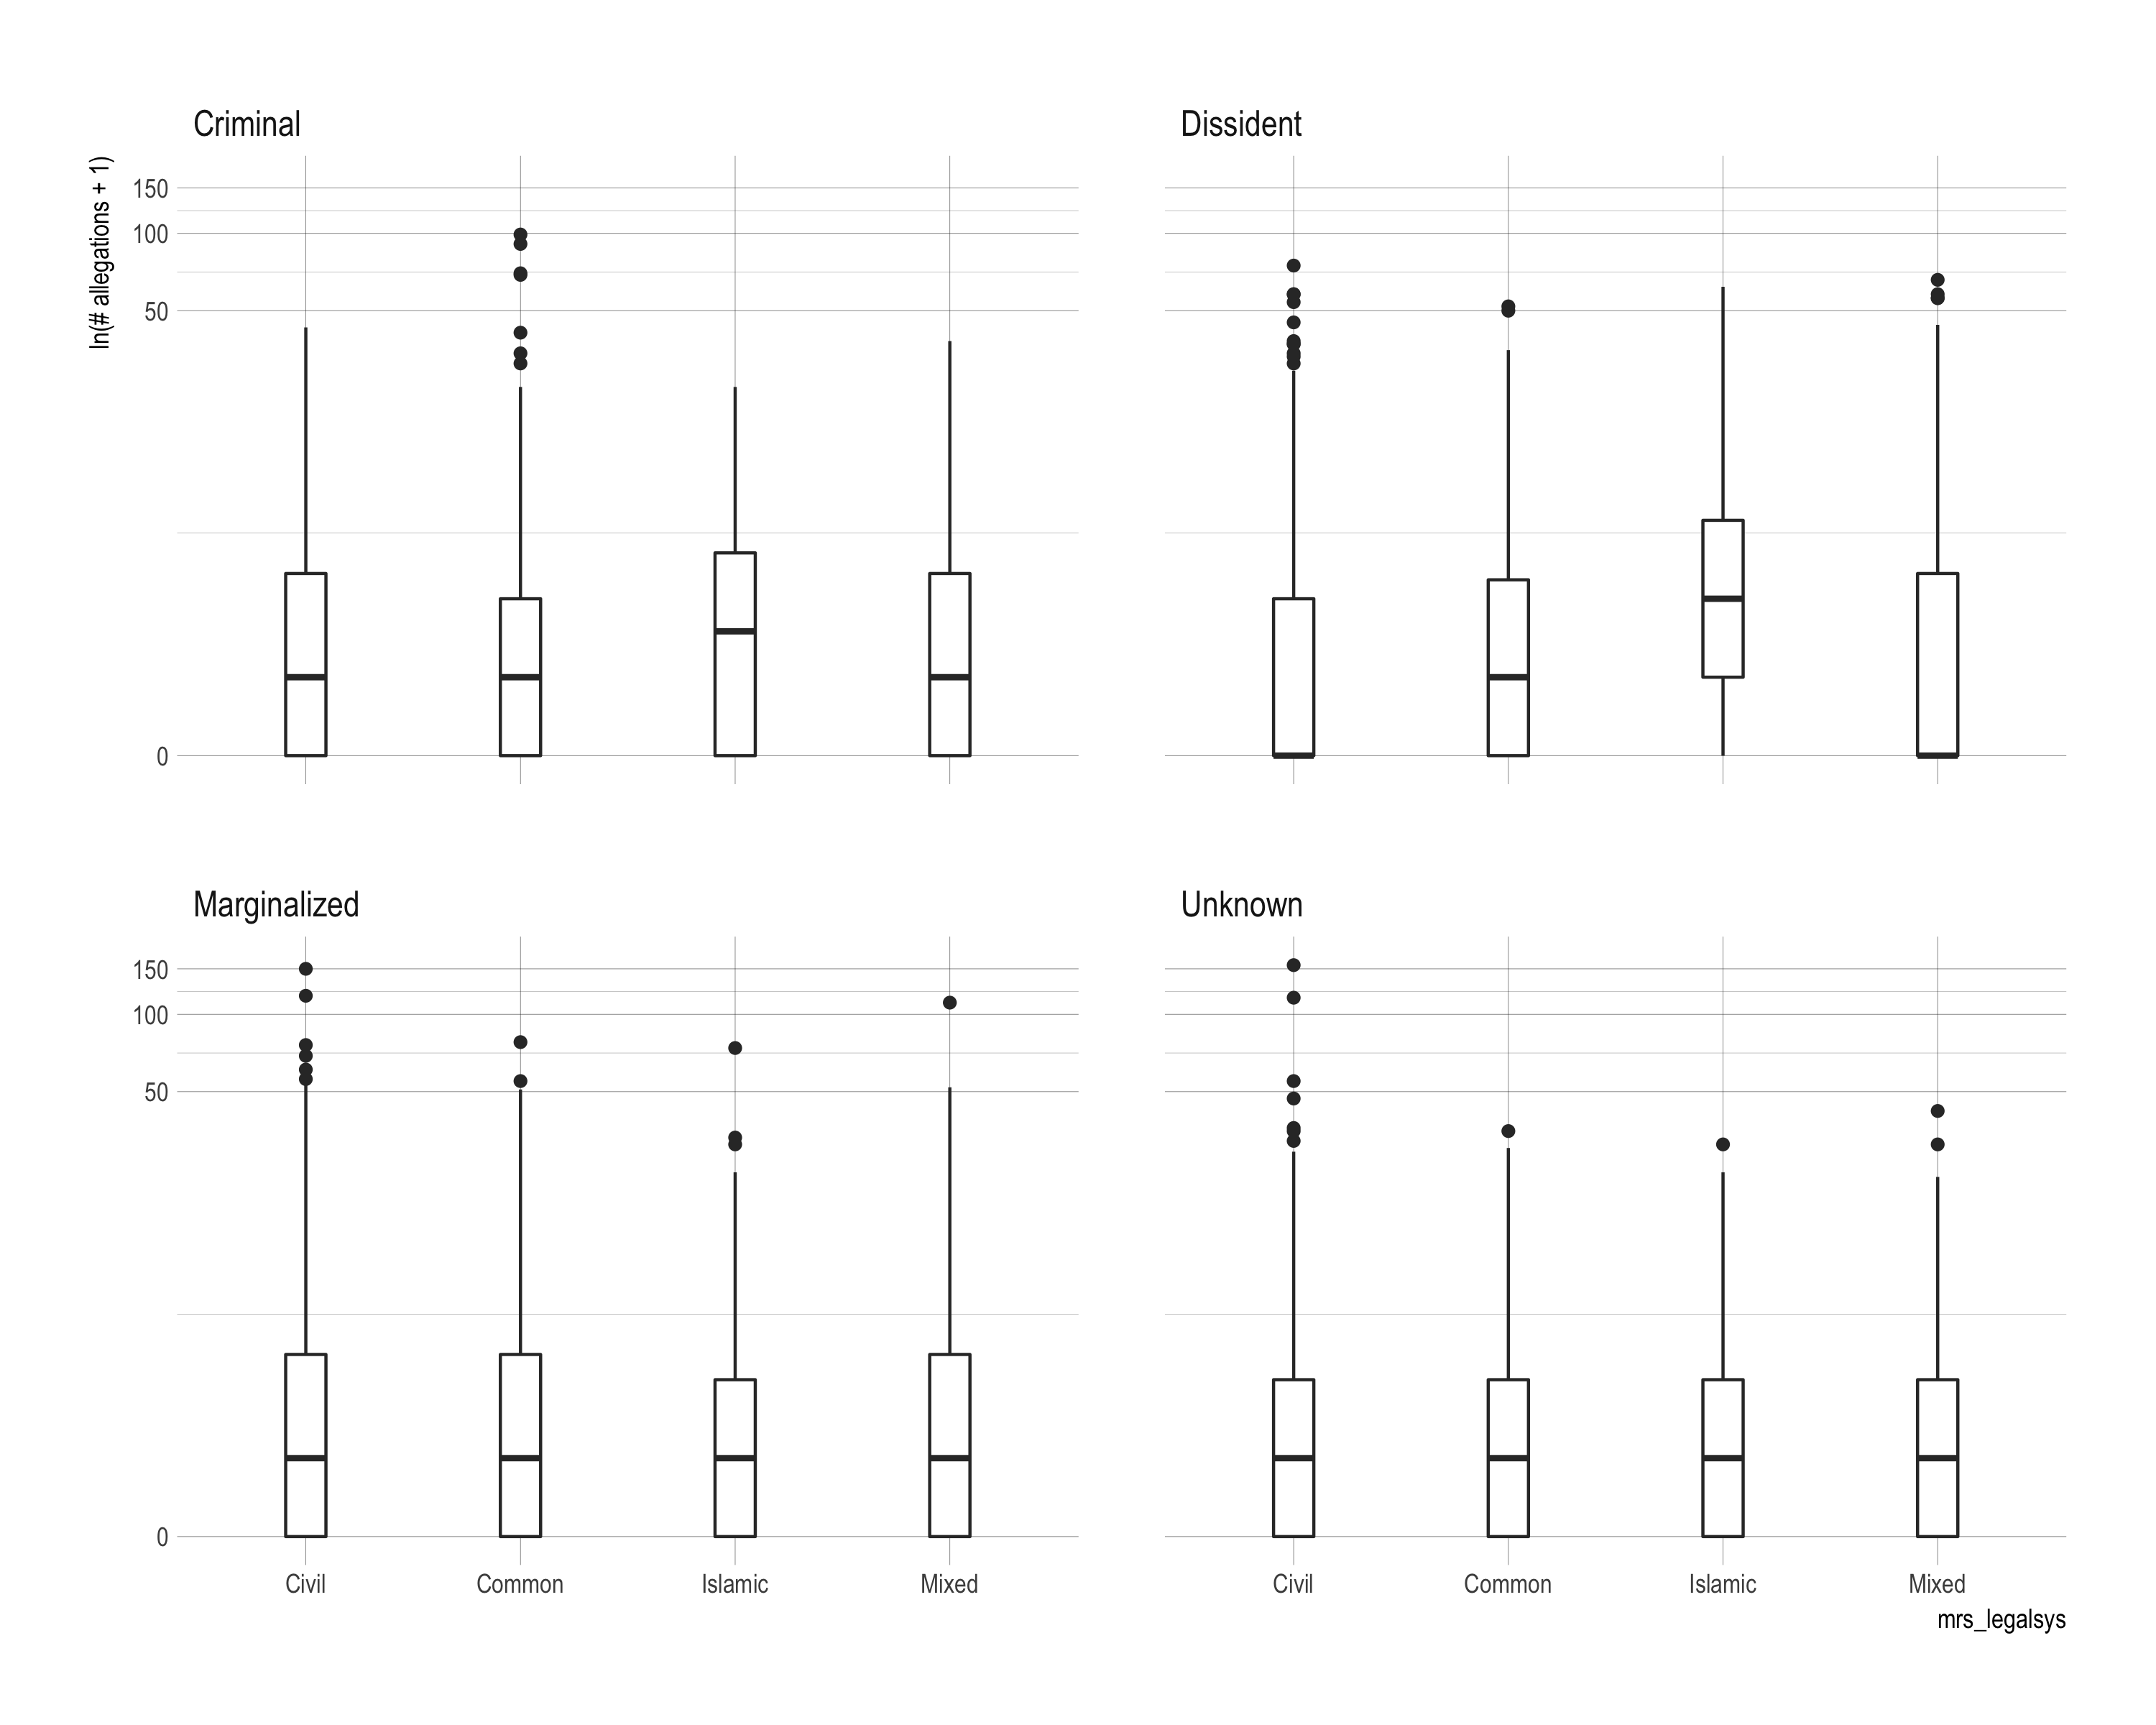
\includegraphics[width=.7\textwidth]{../output/boxplots-itt-allegations-v-legalsys.png}
\end{center}
\end{figure}

\textbf{Summary}. In our empirical analysis we find that:

\begin{itemize}
\item Allegations of torture of marginalized and criminal victims are as common as allegations that dissidents are tortured.
\item However, the number of allegations that a country tortures one kind of victim are only loosely correlated with allegations for other kinds of victims. In other words, states often don't torture the same kinds of victims, or at least are not alleged to do so.
\item Judicial independence is related to a slighly lower number of allegations that dissidents are tortured, but not of abuse of criminal and marginalized victims. This bears out in the bivariate analysis and coefficient estimates, but not clearly in terms of model fit (no in the random intercept count models, but yes in the machine learing model). 
\item Democracies face fewer allegations of torture of dissidents, but similar levels of accusations that they torture marginalized and criminal victims as dictatorships. There is some indirect evidence that changes to a democratic regime reduce torture allegations within a country.
\item Although judicial independence is higher in democratic regimes, especially parliamentary democracies, its protective effect is in addition to the reduction of dissident torture allegation in democracies, and holds when accounting for regime type. 
\item There is no evidence of a difference in torture allegations between civil, common law, Islamix, and mixed legal system. 
\item Wealth and democracy overall have a stronger relationship to torture allegations than judicial independence, but none of them are good explaining why allegations change within a country over time.
\end{itemize}

\section*{Conclusion}

Our empirical results show that the institutional factors we examined--judicial independence, legal system types, and regime type more generally--have relatively small impacts on the number of torture allegations against differnet types of victims. One caveat is that by including country random intercepts in our models, and thus accounting for between country variation, we have stacked the odds against finding strong assocations. Institutional characteristics usually evolve relatively slowly over time, yet this is what our models concentrate on looking for. Indeed, if we were to exclude country intercepts, we would probably find stronger apparent relationships between these factors and torture allegation levels. The flipside however, and benefit of the strategy we adopted, is that we can be more sure that what we have found, namely the protective effects of demoracy and judicial independence on reduced levels of dissident torture, are not spurious results driven by unmodeled and unobserved differences between countries. 

A logical follow up would be to focus explicitly on instances where our variables of interest change within a country and how these changes map onto changes in the levels of torture allegations. This would more clearly support the tentative conclusions we draw in regard to the differences between the count model results and predictive importance for judicial independence and some aspects of democracy that the XGBoost model results hint at. 

Overall, our models leave most of the fluctuation in torture allegation over time unexplained, e.g. it is not clear why allegations spiked in the US and Turkey in the mid to late 1990's for example. It seems reasonable to speculate that internal domestic events, like the Kurdish insurgency in Turkey, are responsible for these spikes. With that in mind, one possibility we have not examined, but which may promise more clear results in respect to judicial and legal factors, is the hypothesis that these factors moderate the impact of adverse events on torture allegations. In other words, is it possible that legal and institutional protections against torture work best by moderating the ability of a state to adopt torture tactics when faced by domestic unrest or rebellion? 

\clearpage
\begin{singlespace}
\bibliographystyle{apsr}
\bibliography{beg_hil}
\end{singlespace}

\end{document}


oversight and punishment
	courts of law
	explicit prohibition on torture/cruel punishment
	no punishment without law
	prison registry
	corporal punishment ban
	false imprisonment

reduce incentive to use torture in criminal investigation
	evidence
	miranda

minimize opportunities for abuse by limiting time in detention 
	pre-trial release
	habeas corpus
	due process
	speedy trial
		
create evidentiary obstacles for securing a criminal conviction
	jury trial 
	examine witnesses
	common law system is a rough proxy for adversarial trial system in which court takes no active part in criminal investigation 
	fair trial
	presumption of innocence
	miranda	
	right to counsel
	


